% Version 3.1 December 2024
% See section 11 of the User Manual for version history
%
%%%%%%%%%%%%%%%%%%%%%%%%%%%%%%%%%%%%%%%%%%%%%%%%%%%%%%%%%%%%%%%%%%%%%%
%%                                                                 %%
%% Please do not use \input{...} to include other tex files.       %%
%% Submit your LaTeX manuscript as one .tex document.              %%
%%                                                                 %%
%% All additional figures and files should be attached             %%
%% separately and not embedded in the \TeX\ document itself.       %%
%%                                                                 %%
%%%%%%%%%%%%%%%%%%%%%%%%%%%%%%%%%%%%%%%%%%%%%%%%%%%%%%%%%%%%%%%%%%%%%

%%\documentclass[referee,sn-basic]{sn-jnl}% referee option is meant for double line spacing

%%=======================================================%%
%% to print line numbers in the margin use lineno option %%
%%=======================================================%%

%%\documentclass[lineno,pdflatex,sn-basic]{sn-jnl}% Basic Springer Nature Reference Style/Chemistry Reference Style

%%=========================================================================================%%
%% the documentclass is set to pdflatex as default. You can delete it if not appropriate.  %%
%%=========================================================================================%%

%%\documentclass[sn-basic]{sn-jnl}% Basic Springer Nature Reference Style/Chemistry Reference Style

%%Note: the following reference styles support Namedate and Numbered referencing. By default the style follows the most common style. To switch between the options you can add or remove “Numbered” in the optional parenthesis. 
%%The option is available for: sn-basic.bst, sn-chicago.bst%  
 
%%\documentclass[pdflatex,sn-nature]{sn-jnl}% Style for submissions to Nature Portfolio journals
%%\documentclass[pdflatex,sn-basic]{sn-jnl}% Basic Springer Nature Reference Style/Chemistry Reference Style
%%\documentclass[pdflatex,sn-mathphys-num]{sn-jnl}% Math and Physical Sciences Numbered Reference Style
\documentclass[pdflatex,sn-mathphys-ay]{sn-jnl}% Math and Physical Sciences Author Year Reference Style
%%\documentclass[pdflatex,sn-aps]{sn-jnl}% American Physical Society (APS) Reference Style
%%\documentclass[pdflatex,sn-vancouver-num]{sn-jnl}% Vancouver Numbered Reference Style
%%\documentclass[pdflatex,sn-vancouver-ay]{sn-jnl}% Vancouver Author Year Reference Style
%%\documentclass[pdflatex,sn-apa]{sn-jnl}% APA Reference Style
%%\documentclass[pdflatex,sn-chicago]{sn-jnl}% Chicago-based Humanities Reference Style

%%%% Standard Packages
%%<additional latex packages if required can be included here>

\usepackage{graphicx}%
\usepackage{multirow}%
\usepackage{amsmath,amssymb,amsfonts}%
\usepackage{amsthm}%
\usepackage{mathrsfs}%
\usepackage[title]{appendix}%
\usepackage{xcolor}%
\usepackage{textcomp}%
\usepackage{manyfoot}%
\usepackage{booktabs}%
\usepackage{algorithm}%
\usepackage{algorithmicx}%
\usepackage{algpseudocode}%
\usepackage{listings}%
\usepackage{rotating}%
\usepackage{tikz}
\usetikzlibrary{shapes.geometric, arrows.meta, positioning, calc, fit, backgrounds}


%%%%

%%%%%=============================================================================%%%%
%%%%  Remarks: This template is provided to aid authors with the preparation
%%%%  of original research articles intended for submission to journals published 
%%%%  by Springer Nature. The guidance has been prepared in partnership with 
%%%%  production teams to conform to Springer Nature technical requirements. 
%%%%  Editorial and presentation requirements differ among journal portfolios and 
%%%%  research disciplines. You may find sections in this template are irrelevant 
%%%%  to your work and are empowered to omit any such section if allowed by the 
%%%%  journal you intend to submit to. The submission guidelines and policies 
%%%%  of the journal take precedence. A detailed User Manual is available in the 
%%%%  template package for technical guidance.
%%%%%=============================================================================%%%%

%% as per the requirement new theorem styles can be included as shown below
\theoremstyle{thmstyleone}%
\newtheorem{theorem}{Theorem}%  meant for continuous numbers
%%\newtheorem{theorem}{Theorem}[section]% meant for sectionwise numbers
%% optional argument [theorem] produces theorem numbering sequence instead of independent numbers for Proposition
\newtheorem{proposition}[theorem]{Proposition}% 
%%\newtheorem{proposition}{Proposition}% to get separate numbers for theorem and proposition etc.

\theoremstyle{thmstyletwo}%
\newtheorem{example}{Example}%
\newtheorem{remark}{Remark}%

\theoremstyle{thmstylethree}%
\newtheorem{definition}{Definition}%

\raggedbottom
%%\unnumbered% uncomment this for unnumbered level heads

\begin{document}

\title[Explainable Hotel Cancellation Prediction Models]{Explainable Hotel Booking Cancellation Prediction Models: Towards Trustworthy Survival Analysis in Hospitality}

%%=============================================================%%
%% GivenName	-> \fnm{Joergen W.}
%% Particle	-> \spfx{van der} -> surname prefix
%% FamilyName	-> \sur{Ploeg}
%% Suffix	-> \sfx{IV}
%% \author*[1,2]{\fnm{Joergen W.} \spfx{van der} \sur{Ploeg} 
%%  \sfx{IV}}\email{iauthor@gmail.com}
%%=============================================================%%

\author*[1]{\fnm{Mustafa} \sur{Cavus}}\email{mustafacavus@eskisehir.edu.tr}

%\author[2,3]{\fnm{Second} \sur{Author}}\email{iiauthor@gmail.com}
%\equalcont{These authors contributed equally to this work.}

%\author[1,2]{\fnm{Third} \sur{Author}}\email{iiiauthor@gmail.com}
%\equalcont{These authors contributed equally to this work.}

\affil[1]{\orgname{Eskisehir Technical University}, \orgdiv{Department of Statistics}, \postcode{26555}, \city{Eskisehir}, \country{Türkiye}}

%\affil[2]{\orgdiv{Department}, \orgname{Organization}, \orgaddress{\street{Street}, \city{City}, \postcode{10587}, \state{State}, \country{Country}}}

%\affil[3]{\orgdiv{Department}, \orgname{Organization}, \orgaddress{\street{Street}, \city{City}, \postcode{610101}, \state{State}, \country{Country}}}

%%==================================%%
%% Sample for unstructured abstract %%
%%==================================%%

\abstract{Hotel booking cancellations impose significant operational and financial risks on revenue management systems, traditionally addressed through static binary classification models. Such approaches fail to capture the temporal dynamics of cancellation behaviors—specifically, \textit{when} a cancellation is most likely to occur between the booking date and check-in. This study addresses this critical gap by formulating cancellation prediction as a survival analysis problem. We benchmark a diverse ensemble of machine learning survival models—including Cox Proportional Hazards, Random Survival Forests, Oblique Random Survival Forests, and Conditional Survival Forests—across two distinct hotel booking datasets with contrasting structural feature spaces. Our findings demonstrate that while standard Random Survival Forests achieve high discriminative rankings, Oblique Random Survival Forests and Conditional Survival Forests deliver superior probability calibration. Furthermore, to advance trustworthy artificial intelligence in hospitality, we integrate time-dependent XAI techniques—Survival Permutation Feature Importance and Partial Dependence Survival Profiles. These tools uncover the non-linear, time-varying influence of core attributes such as \textit{lead time}, \textit{average daily rate}, and \textit{deposit policy} on cancellation risk curves. Specifically, the explanations expose an accelerating cancellation hazard close to check-in among premium-priced bookings driven by guest price sensitivity and intertemporal arbitrage, while isolating a structural anomaly where non-refundable reservations display paradoxically depressed survival rates due to speculative group allocations. The resulting framework equips revenue managers with transparent decision intelligence to dynamically optimize overbooking limits, calibrate cancellation penalties, and mitigate revenue leakage under demand uncertainty.}

\keywords{hotel booking cancellation, XAI, survival analysis}

\maketitle
%%%%%%%%%%%%%%%%%%%%%%%%%%%%%%%%%%%%%%%%%%%%%%%%%%%
\section{Introduction}
\label{sec:introduction}
    
In the tourism sector, demand forecasting stands as a foundational pillar for strategic capacity management \citep{antonio2017predicting}, resource allocation, and dynamic pricing optimization \citep{ampountolas2025predicting}. Beyond its operational utility, predictive modeling in hospitality functions as a mechanism that converts raw transactional data into strategic intelligence, enabling industry stakeholders and policymakers to formulate competitive strategies and narrow the structural gap between projected supply and realized demand \citep{herrera2024machine}. Unlike traditional inventory-based businesses, hotel room reservations represent highly perishable services where an unallocated room on any given calendar night results in an absolute loss of potential revenue \citep{antonio2019big}, meaning hotels cannot recover the value of unsold capacity once a night passes \citep{mir2026decoding}. Consequently, revenue management (RM) departments rely on predictive analytics to maintain occupancy levels \citep{yoo2024predicting} and capture maximum market value through dynamic inventory controls \citep{liu2025explainable}. However, the accuracy of short-term demand signals is fundamentally distorted by hotel booking cancellations. These cancellations compromise forecasting reliability \citep{liu2023hospitality, luo2025hotel} and account for operational losses estimated at approximately 20\% of hotel revenues \citep{sierag2015revenue, falk2018modelling}.
    
The widespread adoption of online travel agencies and digital booking channels has structurally altered consumer behavior by introducing high price transparency and lowering the transactional barriers to canceling previously confirmed reservations. Prospective travelers frequently exhibit opportunistic behaviors, using flexible policies to secure multiple alternatives \citep{chen2023prediction} or engaging in intertemporal arbitrage by rebooking when lower rates emerge \citep{mir2026decoding} closer to their scheduled arrival date \citep{ampountolas2025predicting}. To hedge against this persistent operational risk, hotels conventionally enforce restrictive, non-refundable penalty windows \citep{yang2024predicting} or deploy overbooking quotas \citep{antonio2017predicting}. Nevertheless, these traditional practices often yield negative externalities, such as eroding customer satisfaction, triggering high relocation costs, and damaging the brand reputation of the property in competitive digital ecosystems \citep{falk2018modelling}. To circumvent the adverse consequences of blanket restrictions, revenue managers increasingly rely on predictive models to estimate individual booking cancellation probabilities, enabling personalized retention actions and granular capacity controls \citep{antonio2017predicting, liu2023hospitality, talal2025hotel}.

Within this context, positioning the cancellation problem correctly within the predictive modeling architecture is crucial. Because reservation commitments evolve dynamically as the arrival date approaches, effective revenue management requires continuous monitoring of cancellation hazards rather than static risk snapshots. Nevertheless, traditional hotel booking cancellation prediction studies generally frame the task as static binary classification, focusing solely on predicting whether a booking will ultimately be canceled. This conventional framing inherently ignores the temporal progression of cancellation risks and introduces systematic predictive bias when applied to reservations that remain active in the system with future check-in dates. In historical reservation cohorts, such incomplete observations constitute right-censored data that require time-to-event approaches rather than static classification \citep{kleinbaum2012survival, langbein2025interpretable}. As conceptually illustrated in Figure~\ref{fig:motivation}, survival analysis models resolve this fundamental bias by mathematically integrating right-censored records into the likelihood framework \citep{kovalev2020survlime, langbein2025interpretable}. Crucially, by estimating both the continuous survival trajectory and the instantaneous hazard rate over time, time-to-event modeling provides hospitality enterprises with an actionable roadmap. Predicting precisely \textit{when} an attrition event is most probable enables revenue management systems to dynamically adjust overbooking quotas, determine optimal re-marketing windows for perishable rooms before demand decays \citep{mir2026decoding}, and deploy proactive retention interventions at minimal mitigation cost \citep{antonio2017predicting, ampountolas2025predicting}.

Despite these evident benefits, the practical adoption of sophisticated machine learning survival algorithms—such as Random Survival Forests (RSF), gradient-boosted survival trees, and regularized Cox ensembles—is substantially hindered by their \textit{black-box} complexity. As the hospitality industry increasingly delegates high-stakes forecasting, capacity allocation, and pricing decisions to artificial intelligence, the imperative for Responsible and Trustworthy AI becomes paramount \citep{khan2025artificial}. High-capacity predictive systems that operate opaquely pose severe ethical and operational vulnerabilities, undermining stakeholder trust and managerial accountability \citep{thiebes2021trustworthy, meske2022explainable}. In competitive hospitality ecosystems, managers are rightfully reluctant to deploy automated models whose temporal forecasts cannot be interpreted, audited, or aligned with domain logic. While Explainable Artificial Intelligence (XAI) frameworks have achieved widespread success in explaining static classifiers, explaining time-to-event predictions introduces distinct mathematical challenges due to the continuous and multi-dimensional nature of survival trajectories.

To bridge these critical gaps and operationalize trustworthy AI principles within hospitality management, this paper introduces an end-to-end explainable time-to-event modeling framework. To the best of our knowledge, this is the first study in hospitality revenue management that couples advanced machine learning survival models with continuous, time-dependent global XAI tools. Specifically, this research delivers three principal contributions to literature and practice:
\begin{enumerate}
\item We transcend static binary classification by reframing hotel cancellation forecasting as a continuous time-to-event survival analysis problem, benchmarking 10 survival algorithms across two structurally distinct empirical datasets and demonstrating that Oblique Random Survival Forests and Conditional Survival Forests achieve superior probability calibration for operational risk management.
\item We introduce time-dependent XAI methods—specifically Survival Permutation Feature Importance and Partial Dependence Survival Profiles—to the hospitality domain, tracking the evolving marginal impact of reservation attributes over the booking window to reveal compounding price elasticity near arrival and unmask policy-driven structural anomalies.
\item We bridge algorithmic machine learning outputs with actionable decision support for hotel revenue managers, translating transparent and auditable survival curves into dynamic overbooking quotas, optimal room re-marketing windows, and responsible AI governance.
\end{enumerate}

\section{Related Work}
\label{sec:related_work}

The literature on hotel booking cancellation prediction has evolved from classical statistical models to machine learning classifiers, and recently, toward survival analysis frameworks and interpretability methods. This section reviews these developments under three thematic categories.

\subsection{Machine Learning Classifiers and Feature Interactions}
Early predictions of hotel booking cancellations relied on classification models trained on historical property management system (PMS) data. \cite{antonio2017predicting} applied data mining techniques and decision trees to reservation data from resort and city hotels, demonstrating that individual booking cancellations could be predicted with over 90\% accuracy. Following this, \cite{falk2018modelling} used a probit model on a multi-hotel dataset to identify booking channels as primary determinants of cancellation, showing that online travel agency reservations exhibit significantly higher cancellation rates than traditional bookings. Concurrently, \cite{satu2020performance} conducted a systematic evaluation of preprocessing pipelines for cancellation classifiers, comparing algebraic feature transformation strategies against targeted variable selection. Their results revealed that dimensionality reduction through deliberate feature selection consistently outperformed transformation-based approaches in predictive accuracy, highlighting the critical role of parsimonious input design when modeling reservation-level outcomes.

Subsequent studies focused on expanding feature spaces and modeling non-linear interactions. \cite{antonio2019big} combined PMS records with external indicators, such as weather conditions and pricing trends, showing that incorporating external features improves net demand forecasting. To capture non-linear dependencies without losing interpretability, \cite{chen2023prediction} proposed a hybrid framework combining machine learning classifiers with Bayesian networks. In parallel, researchers focused on business-oriented metrics rather than standard classification accuracy. \cite{liu2023hospitality} developed a profit-driven prediction framework to optimize the financial returns of customer retention campaigns. \cite{liu2025explainable} extended this by proposing a heterogeneous stacking ensemble model designed to maximize revenue under different mitigation costs.

Model benchmarks also shifted toward ensemble architectures. \cite{yoo2024predicting} evaluated multiple classifiers and demonstrated that gradient-boosted tree architectures achieve substantially higher discriminative power than conventional parametric classifiers for cancellation detection. \cite{yang2024predicting} integrated decision trees with feed-forward neural networks to model tabular reservation data, while \cite{luo2025hotel} applied gradient boosting to large-scale datasets, confirming lead time and deposit type as key predictive features. Similarly, \cite{febrian2024hotel} demonstrated the performance advantages of boosting paradigms to capture non-linear booking dynamics. Recently, \cite{ampountolas2025predicting} analyzed a five-year booking dataset and addressed the trade-off between precision and recall by proposing a hybrid model combining gradient boosting and Ridge regression to minimize false negative rates.

\subsection{XAI in Hospitality Prediction}
Because hospitality operations require transparent decision-making, recent studies have integrated post-hoc explainability methods into cancellation models to extract domain-specific insights. \cite{gomez2025machine} used SHAP to interpret global and local feature impacts in hotel booking models, establishing that lead time, special requests, and historical cancellations have non-linear effects on final predictions.
\cite{herrera2024machine} applied TreeSHAP to tree-based ensemble models, revealing that the distribution channel and lead time are the primary
contributors to the predicted cancellation risk across distinct seasonal cohorts.

To balance predictive performance and model understandability, recent architectures combine stacking ensemble models with multi-method explanations. \cite{talal2025hotel} developed a stacked generalization meta-model achieving 96\% prediction accuracy and mapped global and local feature contributions using Kernel SHAP, Tree SHAP, and LIME. Their analysis showed how variables like customer type and deposit requirements interact at an individual level to escalate cancellation probabilities. 

Furthermore, explainability has been linked directly to financial decision-making in hospitality operations. \cite{liu2025explainable} proposed a heterogeneous stacking classifier. They combined global SHAP values with profit-sensitive permutation feature importances, showing that a variable's contribution to classification accuracy does not guarantee a proportional impact on the economic value of retention interventions, thereby underscoring a disconnect between statistical importance and operational profitability. 

Despite these advancements, standard XAI methods in the hospitality literature are restricted to static classification models. They explain whether a booking will cancel, but fail to explain when the risk shifts over time. This limitation has motivated the integration of survival analysis explainers, which translate static predictions into dynamic risk curves.

\subsection{Survival Analysis and Time-to-Event Modeling}
Unlike binary classifiers that treat active bookings as non-canceled (introducing right-censoring bias), survival analysis models time-to-event data mathematically. \cite{kovalev2020survlime} developed SurvLIME, which explains survival models locally by approximating cumulative hazard functions using a Cox proportional hazards formulation. To resolve time-dependent variations in feature effects, \cite{krzyzinski2023survshapt} introduced SurvSHAP(t), a model-agnostic framework that calculates time-dependent Shapley values for survival functions. This framework enables the measurement of how a single feature's influence changes or reverses over a continuous time axis. \cite{langbein2025interpretable} unified these methods for machine learning survival analysis, establishing protocols for auditing complex models in censored data environments.

In the tourism economics domain, \cite{mir2026decoding} applied survival analysis and linear probability models to a longitudinal dataset of over two million bookings. Their empirical findings revealed that guests frequently treat cancellation as a deliberate, utility-maximizing response to evolving market conditions, systematically leveraging flexible refund clauses and monitoring rate fluctuations to rebook at more favorable terms. This evidence confirms the necessity of using time-dependent hazard rate modeling rather than static classification to optimize capacity and RM in hotels.

%%%%%%%%%%%%%%%%%%%%%%%%%%%%%%%%%%%%%%%%%%%%%%%%%%%
\section{Methodology} %%%%%%%%%%%%%%%%%%%%%%%%%%%%%
%%%%%%%%%%%%%%%%%%%%%%%%%%%%%%%%%%%%%%%%%%%%%%%%%%%
\label{sec:methodology}



This section formalizes the time-to-event learning problem in the context of hotel booking cancellations and introduces the two XAI techniques deployed to interpret the trained survival models. Figure~\ref{fig:motivation} conceptually illustrates the fundamental distinction between static binary classification and the survival modeling paradigm adopted in this study.

\begin{figure}[htbp]
\centering
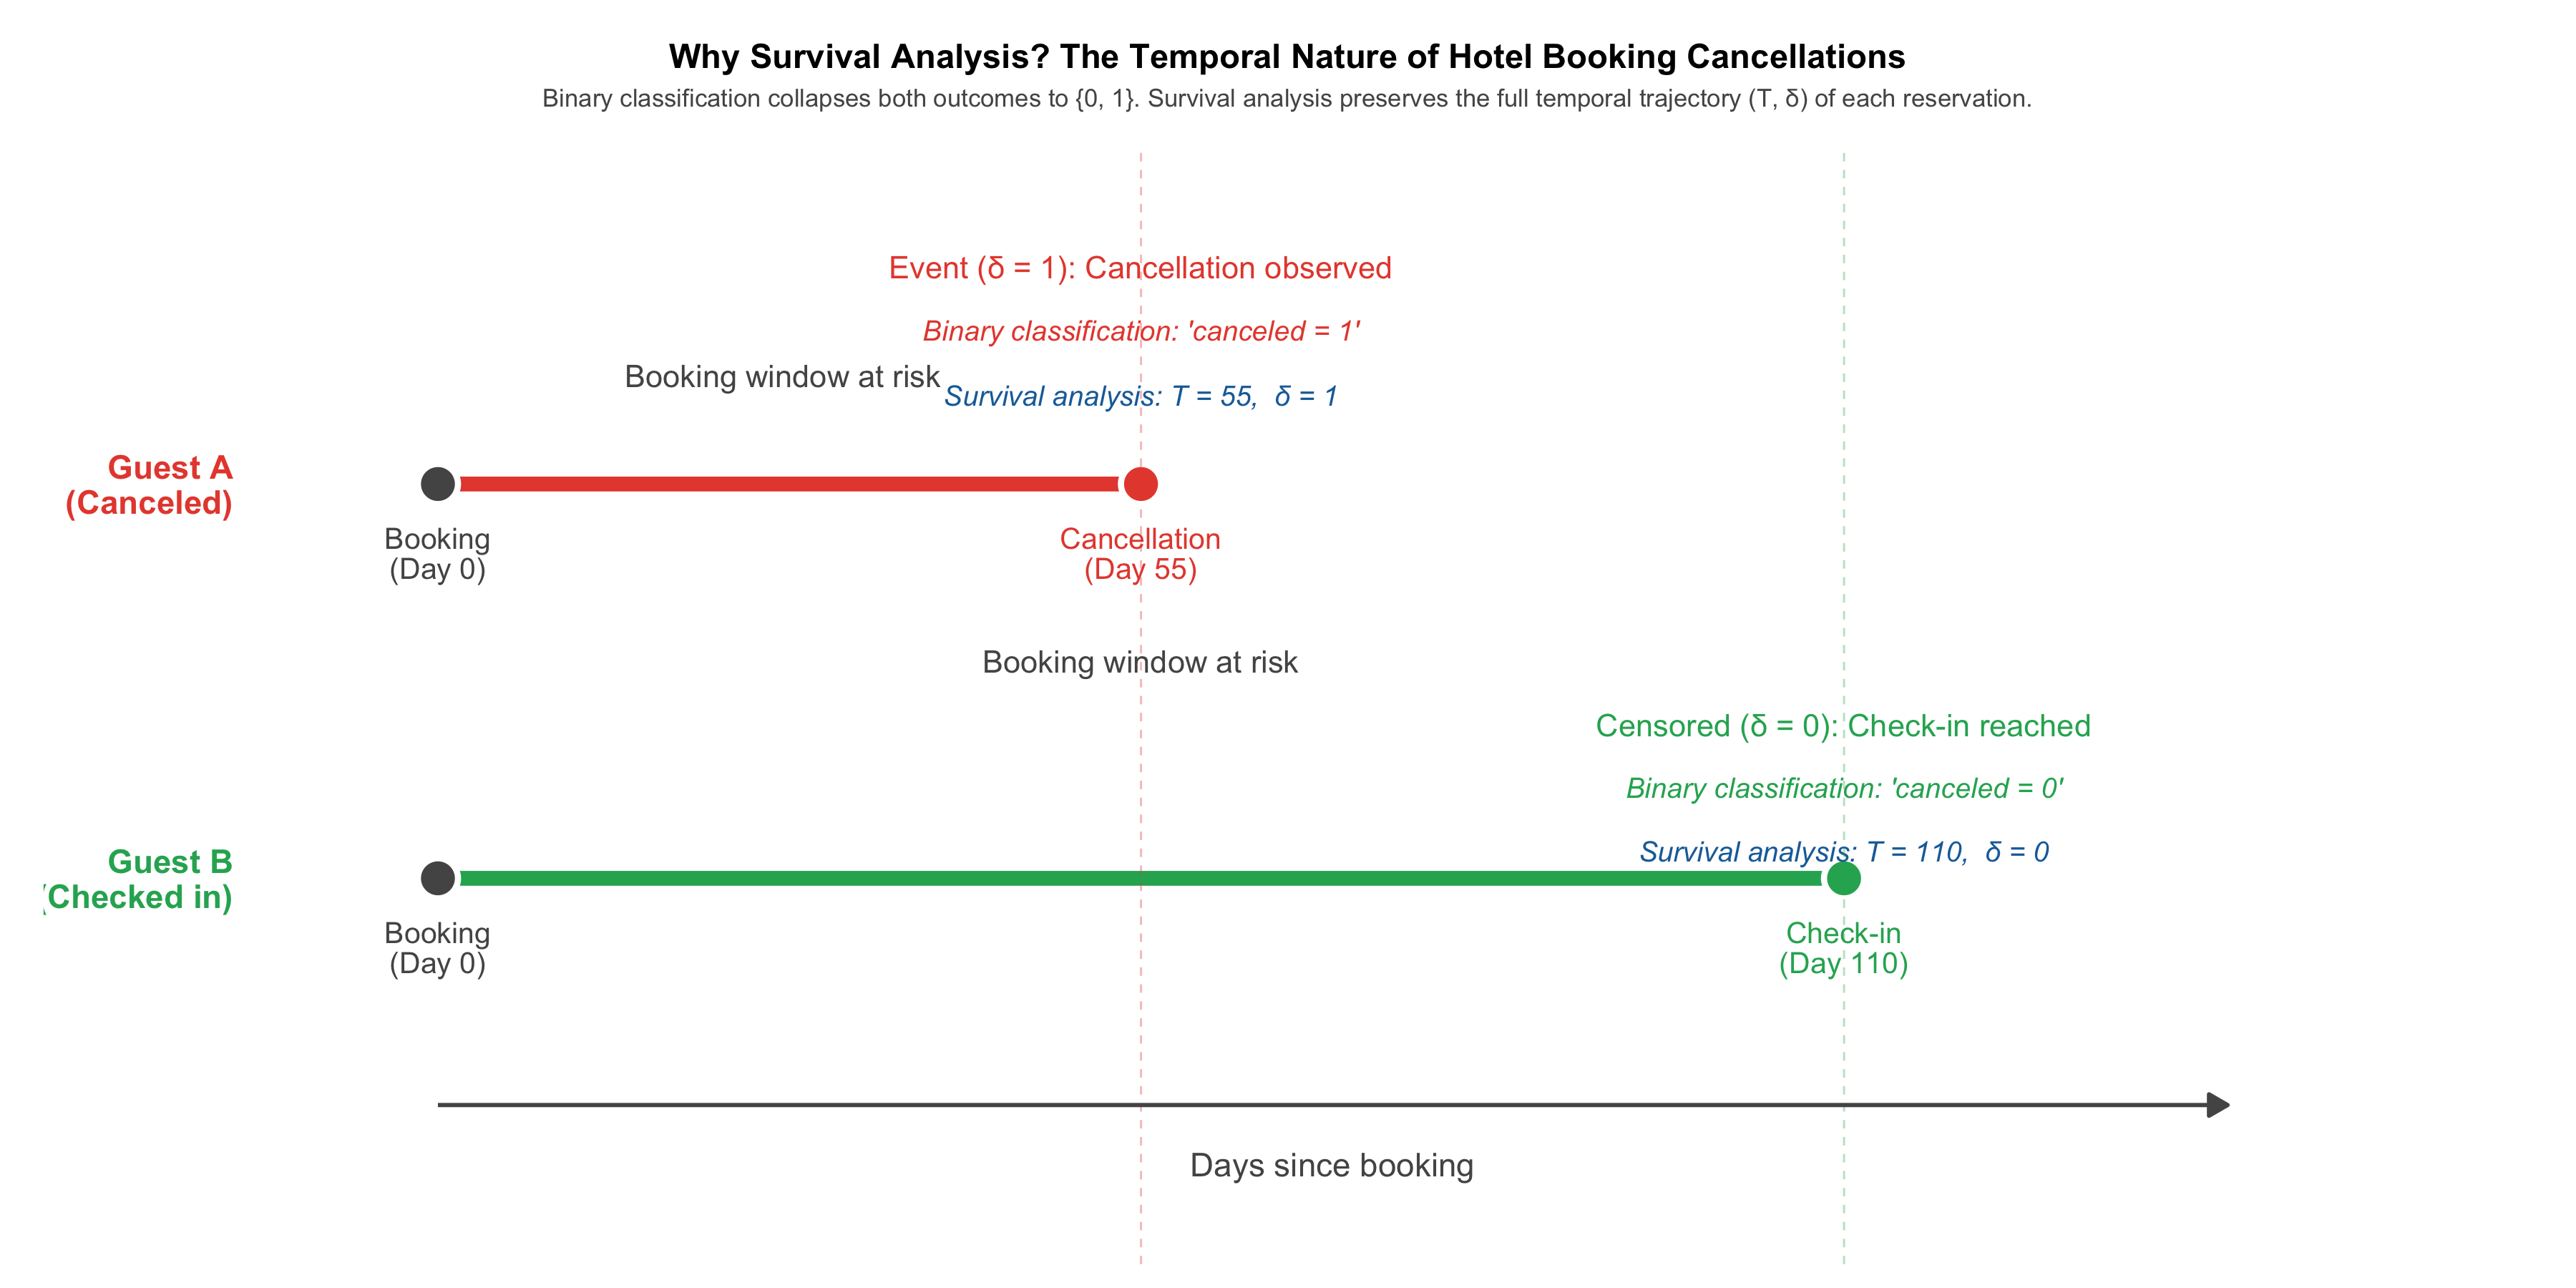
\includegraphics[width=0.95\textwidth]{fig_motivation.png}
\caption{Conceptual comparison of binary classification and survival analysis for hotel booking cancellations. Binary classification reduces both outcomes to a single binary label, discarding the temporal trajectory. Survival analysis preserves the full (Y, $\delta$) pair, enabling dynamic risk estimation over the booking window.}\label{fig:motivation}
\end{figure}

\subsection{Time-to-Event Problem Formulation}

For a given $p$-dimensional feature vector $X \in \mathbb{R}^p$, the conditional survival function $S(t \mid X)$, which models the probability of a reservation remaining active beyond time $t$, is defined as:
\begin{equation}
S(t \mid X) = P(T > t \mid X)
\end{equation}
Correspondingly, the conditional hazard rate $\lambda(t \mid X)$, expressing the instantaneous rate of cancellation at time $t$ given survival up to that point, is formulated as:
\begin{equation}
\lambda(t \mid X) = \lim_{\Delta t \to 0} \frac{P(t \le T < t + \Delta t \mid T \ge t, X)}{\Delta t} = -\frac{d}{dt} \ln S(t \mid X)
\end{equation}
By modeling $\hat{S}(t\mid X)$ directly using machine learning survival algorithms, we dynamically capture how cancellation risk changes over time.

\subsection{Survival Partial Dependence Plots}
To capture the global marginal effect of a specific feature on the predicted survival probability across a continuous time horizon, we employ Survival Partial Dependence Plots (SurvPDP) proposed by \cite{langbein2025interpretable}, which generalizes the classical Partial Dependence Plot (PDP) originally formulated for tabular classification and regression by \cite{friedman2001greedy} to the time-to-event setting. Let $X$ represent the feature vector of size $p$, partitioned into a target feature of interest $X^S$ and the remaining features $X^C$ such that $X = (X^S, X^C)$. The survival function estimated by a machine learning survival model at time $t$ for a given feature configuration is denoted as $\hat{S}(t \mid X)$. The SurvPDP function for $X^S$ at time $t$ is defined by marginalizing over the joint distribution of $X^C$:
\begin{equation}
\text{SurvPDP}(t, x^S) = E_{X^C} \left[ \hat{S}(t \mid (x^S, X^C)) \right] \approx \frac{1}{N} \sum_{i=1}^N \hat{S}\left(t \mid (x^S, x_i^C)\right)
\end{equation}
where $N$ is the number of observations in the dataset, and $x_i^C$ represents the values of the confounding features for the $i$-th instance. By plotting $\text{SurvPDP}(t, x^S)$ across a range of values for $x^S$ and continuous time steps $t$, we can visualize how the marginal survival curves and instantaneous cancellation risks evolve dynamically over the reservation lifecycle.

\subsection{Survival Permutation Feature Importance}
To quantify the global impact of individual features on the survival model's overall predictive performance, we utilize Survival Permutation Feature Importance (SurvPFI) proposed by \cite{langbein2025interpretable}. This framework extends the foundational Permutation Feature Importance (PFI) method originally introduced for tabular data by \cite{breiman2001random} into survival analysis by evaluating time-dependent loss functions. It measures the degradation in a model's predictive performance when the relationship between a target feature $X^j$ and the survival outcomes is broken via random shuffling. 

Let $L(\hat{S}, D)$ represent a loss function (e.g., the IBS or 1 minus Harrell's concordance index) computed for the model $\hat{S}$ on the dataset $D = \{(X_i, Y_i, \delta_i)\}_{i=1}^N$. Let $D^{\pi, j}$ denote the perturbed dataset where the values of feature $X^j$ have been randomly permuted across observations while keeping all other features and target variables $(Y, \delta)$ intact. The permutation feature importance for feature $X^j$ is formulated as:
\begin{equation}
\text{SurvPFI}(X^j) = L(\hat{S}, D^{\pi, j}) - L(\hat{S}, D)
\end{equation}
Alternatively, it can be defined as the ratio $L(\hat{S}, D^{\pi, j}) / L(\hat{S}, D)$. Higher values of $\text{SurvPFI}(X^j)$ indicate that the model relies heavily on feature $X^j$ to predict time-to-event outcomes accurately. In this study, we compute the loss metric based on time-dependent performance criteria to capture the temporal accuracy of booking cancellations.


\begin{figure}[htbp]
\centering
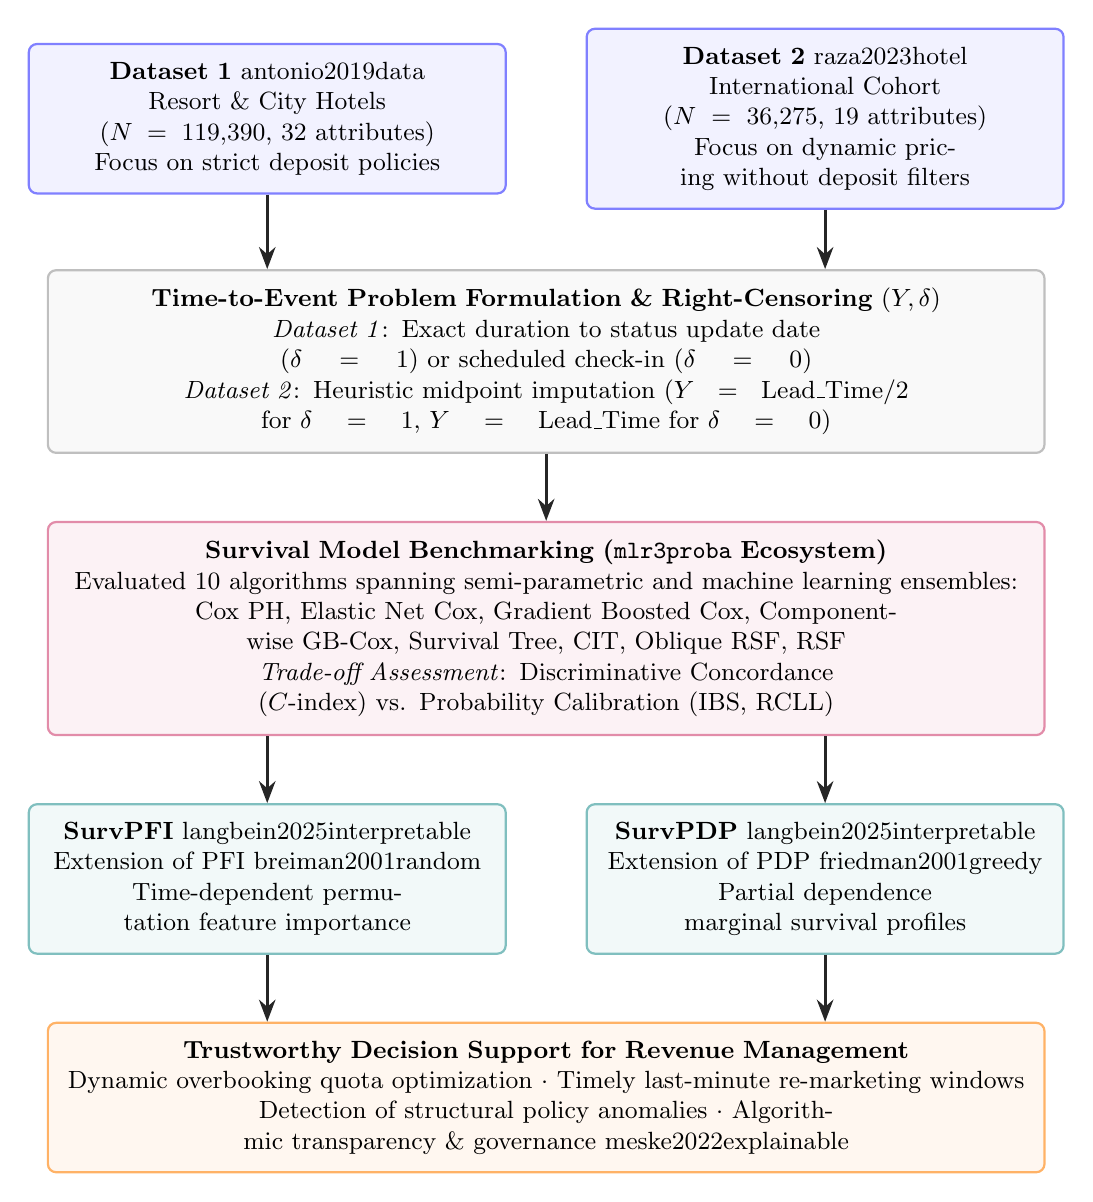
\begin{tikzpicture}[
    >=Stealth,
    every text node part/.style={align=center},
    basebox/.style={
        rectangle, 
        draw=black!75, 
        rounded corners=3pt, 
        font=\small, 
        inner sep=6.5pt,
        fill=white,
        line width=0.8pt
    },
    databox/.style={
        basebox, 
        fill=blue!5, 
        draw=blue!50, 
        text width=5.6cm
    },
    procbox/.style={
        basebox, 
        fill=gray!5, 
        draw=gray!50, 
        text width=12.2cm
    },
    modelbox/.style={
        basebox, 
        fill=purple!5, 
        draw=purple!45, 
        text width=12.2cm
    },
    xaibox/.style={
        basebox, 
        fill=teal!5, 
        draw=teal!50, 
        text width=5.6cm
    },
    outbox/.style={
        basebox, 
        fill=orange!6, 
        draw=orange!60, 
        text width=12.2cm
    },
    arrowline/.style={
        ->, 
        draw=black!85, 
        line width=1.1pt
    }
]

% 1. Datasets
\node[databox] (d1) {\textbf{Dataset 1} \citep{antonio2019data}\\ Resort \& City Hotels ($N=119{,}390$, 32 attributes)\\ Focus on strict deposit policies};
\node[databox, right=1.0cm of d1] (d2) {\textbf{Dataset 2} \citep{raza2023hotel}\\ International Cohort ($N=36{,}275$, 19 attributes)\\ Focus on dynamic pricing without deposit filters};

% Midpoint coordinate
\coordinate (d_mid) at ($(d1.south)!0.5!(d2.south)$);

% 2. TTE Formulation
\node[procbox, below=0.85cm of d_mid] (tte) {
    \textbf{Time-to-Event Problem Formulation \& Right-Censoring $(Y, \delta)$}\\
    \textit{Dataset 1}: Exact duration to status update date ($\delta=1$) or scheduled check-in ($\delta=0$)\\
    \textit{Dataset 2}: Heuristic midpoint imputation ($Y = \text{Lead\_Time}/2$ for $\delta=1$, $Y = \text{Lead\_Time}$ for $\delta=0$)
};

% 3. Benchmarking
\node[modelbox, below=0.85cm of tte] (models) {
    \textbf{Survival Model Benchmarking (\texttt{mlr3proba} Ecosystem)}\\
    Evaluated 10 algorithms spanning semi-parametric and machine learning ensembles:\\
    Cox PH, Elastic Net Cox, Gradient Boosted Cox, Component-wise GB-Cox, Survival Tree, CIT, Oblique RSF, RSF\\
    \textit{Trade-off Assessment}: Discriminative Concordance ($C$-index) vs. Probability Calibration (IBS, RCLL)
};

% 4. XAI Split
\coordinate (m_mid) at (models.south);
\node[xaibox, below left=0.85cm and 0.5cm of m_mid] (pfi) {
    \textbf{SurvPFI} \citep{langbein2025interpretable}\\
    Extension of PFI \citep{breiman2001random}\\
    Time-dependent permutation feature importance
};

\node[xaibox, below right=0.85cm and 0.5cm of m_mid] (pdp) {
    \textbf{SurvPDP} \citep{langbein2025interpretable}\\
    Extension of PDP \citep{friedman2001greedy}\\
    Partial dependence marginal survival profiles
};

% 5. Decision Support
\coordinate (xai_mid) at ($(pfi.south)!0.5!(pdp.south)$);
\node[outbox, below=0.85cm of xai_mid] (out) {
    \textbf{Trustworthy Decision Support for Revenue Management}\\
    Dynamic overbooking quota optimization $\cdot$ Timely last-minute re-marketing windows\\
    Detection of structural policy anomalies $\cdot$ Algorithmic transparency \& governance \citep{meske2022explainable}
};

% --- Arrows with visible clearance and robust line width ---
% From Datasets to TTE
\draw[arrowline] (d1.south) -- (d1.south |- tte.north);
\draw[arrowline] (d2.south) -- (d2.south |- tte.north);

% From TTE to Models
\draw[arrowline] (tte.south) -- (models.north);

% From Models to XAI (Fork)
\draw[arrowline] (models.south -| pfi.north) -- (pfi.north);
\draw[arrowline] (models.south -| pdp.north) -- (pdp.north);

% From XAI to Decision Support
\draw[arrowline] (pfi.south) -- (pfi.south |- out.north);
\draw[arrowline] (pdp.south) -- (pdp.south |- out.north);

\end{tikzpicture}
\caption{Overview of the proposed explainable time-to-event modeling framework. The pipeline proceeds from raw hotel booking data through survival duration construction, multi-algorithm benchmarking, and time-dependent XAI analysis, culminating in trustworthy, actionable insights for RM.}\label{fig:framework}
\end{figure}

\section{Experimental Design} %%%%%%%%%%%%%%%%%%%%%%
%%%%%%%%%%%%%%%%%%%%%%%%%%%%%%%%%%%%%%%%%%%%%%%%%%%
\label{sec:experimental_design}


This section describes the empirical datasets used to validate the proposed framework, details the survival duration construction procedure for each dataset, and outlines the model training and evaluation pipeline. The full experimental workflow is depicted in Figure~\ref{fig:pipeline}.

\subsection{Datasets}
To evaluate the proposed explainable time-to-event frameworks and ensure the generalizability of our findings, we leverage two empirical datasets commonly benchmarked in hospitality demand modeling. The motivation for utilizing two distinct datasets stems from the necessity to test the framework's robustness across diverse structural feature spaces (e.g., the presence versus absence of strict deposit policies). This dual-dataset experimental design demonstrates the capacity of time-dependent XAI tools to adapt to diverse hospitality environments and decode differing market dynamics, such as policy-driven anomalies in one environment versus price-elasticity behaviors in another. Both datasets contain granular, reservation-level transaction records but differ significantly in feature design, sample size, and temporal resolution.

The first dataset, the Hotel Booking Demand dataset (hereafter Dataset 1), was originally introduced by \cite{antonio2019data} and consists of $119,390$ reservations recorded from a Resort Hotel and a City Hotel in Portugal. It contains $32$ variables spanning reservation details, customer demographics, and transactional attributes. The second dataset, the Hotel Reservations dataset (hereafter Dataset 2), was published by \cite{raza2023hotel} and contains $36,275$ observations with $19$ features capturing customer reservation metrics and preferences.

To ensure compatibility with the time-to-event modeling framework, the survival duration ($T$) and censoring indicator ($\delta$) are calculated based on the temporal granularity available. In Dataset 1, the exact survival duration is computed as the number of days elapsed between the booking creation date (arrival date minus lead time) and either the status update date (for confirmed cancellations, $\delta = 1$) or the scheduled check-in date (for active check-outs, $\delta = 0$). Specifically, in the absence of exact timestamps for Dataset 2, we employ a midpoint imputation proxy, setting $Y_i = \text{Lead\_Time}_i / 2$ for canceled bookings ($\delta_i = 1$) under the heuristic assumption of a uniform cancellation risk prior to check-in, and $Y_i = \text{Lead\_Time}_i$ ($\delta_i = 0$) for non-canceled reservations. This constitutes a strong methodological assumption of midpoint imputation, as the precise time of cancellation is unknown. While this heuristic continuous proxy facilitates survival analysis modeling on right-censored data architectures, it is a limitation since it uniformly redistributes cancellation times rather than reflecting natural empirical distributions.

A detailed statistical characterization of all features across both datasets, including their distribution metrics and categories, is structured in Table~\ref{tab:dataset_comparison}.

\begin{table}[htbp]
\caption{Statistical profile and comparison of the datasets}\label{tab:dataset_comparison}
\begin{tabular*}{\textwidth}{@{\extracolsep{\fill}} p{0.34\textwidth} p{0.29\textwidth} p{0.29\textwidth}}
\toprule
Variables & Dataset 1 \citep{antonio2019data} & Dataset 2 \citep{raza2023hotel} \\
\midrule
Observations ($N$) & 119,390 & 36,275 \\
Total Predictors ($p$) & 29 & 17 \\
Target Event Rate (Canceled) & 37.04\% & 32.76\% \\
\midrule
\textit{Continuous} & & \\\midrule
Lead Time (days) & $[0, 737]$ & $[0, 443]$ \\
ADR / Price & $[-6.38, 5400]$ & $[0, 540]$ \\
Weekend Nights & $[0, 19]$ & $[0, 7]$ \\
Week Nights & $[0, 50]$ & $[0, 17]$ \\
\midrule
\textit{Categorical \& Ordinal} & & \\\midrule
Number of Adults & $[0, 55]$ & $[0, 4]$ \\
Number of Children & $[0, 10]$ & $[0, 10]$ \\
Number of Prior Cancellations & $[0, 26]$ & $[0, 13]$ \\
Number of Special Requests & $[0, 5]$ & $[0, 5]$ \\
Number of Booking Modifications & $[0, 21]$ & -- \\
Booking Channel & \{\text{Online}, \text{Offline}, \text{Corporate}, \text{Direct}, \text{Aviation}\} & \{\text{Online}, \text{Offline}, \text{Corporate}, \text{Aviation}\} \\
Deposit Requirement & \{\text{No Deposit}, \text{Non-Refund}, \text{Refundable}\} & -- \\
Selected Meal Plan & \{\text{BB}, \text{FB}, \text{HB}, \text{SC}, \text{Undefined}\} & \{\text{Meal 1}, \text{Meal 2}, \text{Meal 3}, \text{Undefined}\} \\
\midrule
\textit{Survival Schema} & & \\\midrule
Survival Time ($T$ / $Y$) & Actual elapsed days to event/check-in & Imputed duration (Lead Time / 2 for events; Lead Time for censored) \\
Event indicator ($\delta=1$) & Confirmed Cancellation & Canceled Status \\
Censored indicator ($\delta=0$) & Check-in reached & Not Canceled \\
\bottomrule
\end{tabular*}
\end{table}



%%%%%%%%%%%%%%%%%%%%%%%%%%%%%%%%%%%%%%%%%%%%%%%%%%%
\subsection{Model Training and Evaluation Pipeline}
\label{sec:experiments}

To rigorously evaluate the predictive capabilities and generalizability of the survival models, we adopted a nested evaluation design. Both datasets were first partitioned into an internal training partition (80\%) and a completely independent, held-out test partition (20\%) using stratified sampling to strictly preserve the empirical censoring distributions ($\delta$) and event-time densities. The entire experimental pipeline was orchestrated using the \texttt{mlr3proba} ecosystem in R. Within the 80\% training partition, models were trained and internally validated using stratified 10-fold cross-validation to safeguard against overfitting and ensure numerical stability. Following cross-validated model training, final out-of-sample predictive performance was benchmarked on the untouched 20\% held-out test partition across four complementary metrics. Crucially, to reflect true out-of-sample operational conditions and prevent data leakage, all subsequent model explanations (SurvPFI and SurvPDP) were extracted exclusively on this 20\% held-out test partition. The complete experimental workflow is visualized in Figure~\ref{fig:pipeline}.

%%%%%%%%%%%%%%%%%%%%%%%%%%%%%%%%%%%%%%%%%%%%%%%%%%%%%%%%%%%%%%%%%%%%%%%%%%%%%%%%%%%%%%%%%%%%%%%%

\begin{figure}[htbp]
\centering
\resizebox{0.92\textwidth}{!}{
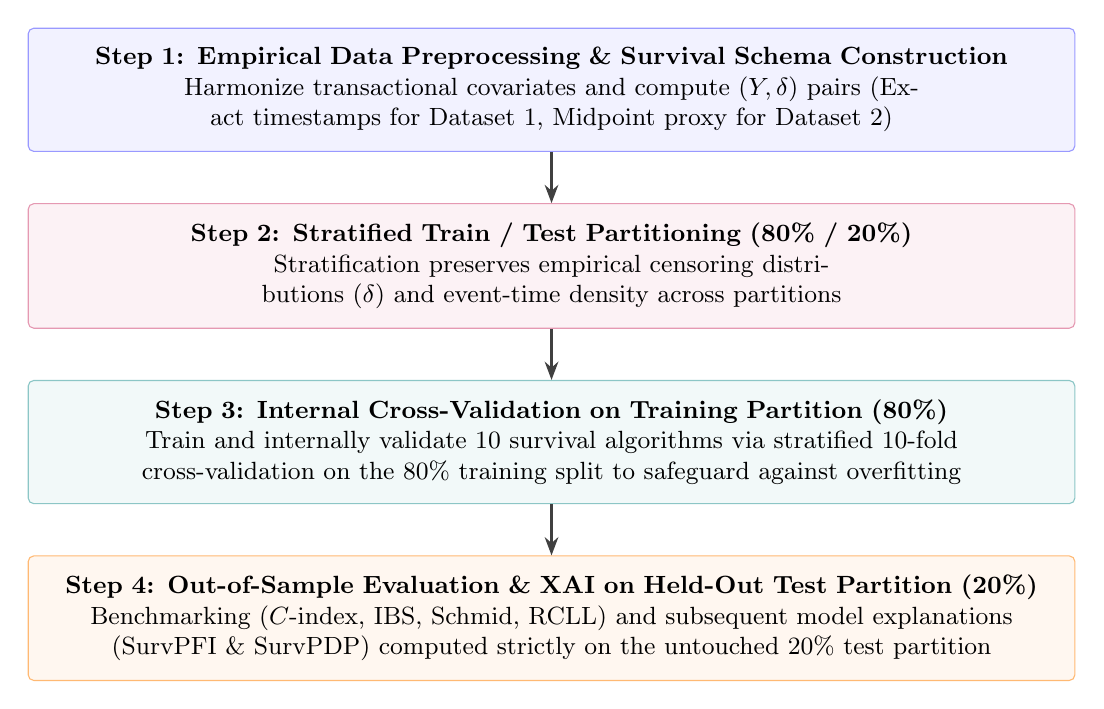
\begin{tikzpicture}[
    >=Stealth,
    node distance=0.65cm,
    every text node part/.style={align=center},
    pipebox/.style={
        rectangle, 
        draw=black!70, 
        rounded corners=2pt, 
        font=\small, 
        inner sep=7pt,
        fill=white,
        text width=12.8cm
    },
    stepbox/.style={
        pipebox,
        fill=blue!5,
        draw=blue!40
    },
    splitbox/.style={
        pipebox,
        fill=purple!5,
        draw=purple!40
    },
    trainbox/.style={
        pipebox,
        fill=teal!5,
        draw=teal!45
    },
    evalbox/.style={
        pipebox,
        fill=orange!6,
        draw=orange!55
    },
    arrowline/.style={
        ->, 
        draw=black!75, 
        line width=0.8pt
    }
]

\node[stepbox] (p1) {
    \textbf{Step 1: Empirical Data Preprocessing \& Survival Schema Construction}\\
    Harmonize transactional covariates and compute $(Y, \delta)$ pairs (Exact timestamps for Dataset 1, Midpoint proxy for Dataset 2)
};

\node[splitbox, below=0.65cm of p1] (p2) {
    \textbf{Step 2: Stratified Train / Test Partitioning (80\% / 20\%)}\\
    Stratification preserves empirical censoring distributions ($\delta$) and event-time density across partitions
};

\node[trainbox, below=0.65cm of p2] (p3) {
    \textbf{Step 3: Internal Cross-Validation on Training Partition (80\%)}\\
    Train and internally validate 10 survival algorithms via stratified 10-fold cross-validation on the 80\% training split to safeguard against overfitting
};

\node[evalbox, below=0.65cm of p3] (p4) {
    \textbf{Step 4: Out-of-Sample Evaluation \& XAI on Held-Out Test Partition (20\%)}\\
    Benchmarking ($C$-index, IBS, Schmid, RCLL) and subsequent model explanations (SurvPFI \& SurvPDP) computed strictly on the untouched 20\% test partition
};

\draw[arrowline] (p1) -- (p2);
\draw[arrowline] (p2) -- (p3);
\draw[arrowline] (p3) -- (p4);

\end{tikzpicture}
}
\caption{Experimental pipeline for model training, evaluation, and explanation. Each dataset undergoes survival duration construction, followed by stratified train/test splitting (80\%/20\%), internal 10-fold cross-validation on the training set, and ultimate out-of-sample evaluation and XAI interpretation strictly on the 20\% held-out test set.}\label{fig:pipeline}
\end{figure}

\section{Results} %%%%%%%%%%%%%%%%%%%%%%%%%%%%%%%%%
%%%%%%%%%%%%%%%%%%%%%%%%%%%%%%%%%%%%%%%%%%%%%%%%%%%


This section presents the empirical findings of the study across two complementary dimensions. First, we compare the predictive performance of the 10 benchmarked survival models using discriminative and calibration metrics. Second, we apply time-dependent XAI tools to interpret the best-performing models and extract actionable temporal insights for hotel RM.

\subsection{Predictive Performance}

In this section, we present a comparative predictive performance evaluation of the 10 survival analysis models on the test partitions of both Dataset 1 and Dataset 2. To capture the multi-dimensional capacity of time-to-event models, we evaluate performance across three distinct criteria:
\begin{enumerate}
\item \textbf{Discriminative Power}: Evaluated using the $C$-index, which measures the model's ability to correctly order individual cancellation event times (i.e., whether a customer predicted to cancel earlier does indeed cancel first).
\item \textbf{Probability Calibration and Accuracy}: Assessed using the IBS and the Integrated Schmid Score. IBS represents the mean squared error between the estimated survival probability and the status over time. The Integrated Schmid Score is an alternative IPCW (Inverse Probability of Censoring Weighting) score that evaluates probability discrepancies under non-uniform censoring regimes.
\item \textbf{Distributional Fit and Likelihood}: Measured via the Right-Censored Log-Likelihood (RCLL), capturing the information gain and likelihood of the observed survival times under the predicted distribution.
\end{enumerate}

Table~\ref{tab:performance_comparison} details the comparative test performance metrics of the models.

\begin{sidewaystable}[htbp]
\centering
\small
\caption{Predictive performance metrics on test partitions of Dataset 1 and Dataset 2}\label{tab:performance_comparison}
\begin{tabular*}{\textwidth}{@{\extracolsep{\fill}} lcccccccc}
\toprule
& \multicolumn{4}{c}{Dataset 1} & \multicolumn{4}{c}{Dataset 2} \\
\cmidrule(lr){2-5} \cmidrule(lr){6-9}
Model & $C$-index $\uparrow$ & IBS $\downarrow$ & Schmid $\downarrow$ & RCLL $\downarrow$ & $C$-index $\uparrow$ & IBS $\downarrow$ & Schmid $\downarrow$ & RCLL $\downarrow$ \\
\midrule
\quad Oblique RSF & 0.7855 & 0.0843 & 0.1999 & \textbf{1.5821} & 0.8108 & 0.0750 & 0.1937 & 0.9908 \\
\quad GB-Cox & 0.7654 & 0.0957 & 0.2033 & 2.0601 & 0.8087 & 0.1170 & 0.2631 & 1.8390 \\
\quad Cond. Forest & 0.7845 & -- & -- & -- & 0.8075 & \textbf{0.0591} & \textbf{0.1571} & 1.1031 \\
\quad Cox PH & 0.7776 & \textbf{0.0842} & \textbf{0.1636} & 2.0268 & 0.8073 & 0.1164 & 0.2430 & 1.8306 \\
\quad CIT & 0.6459 & -- & -- & -- & 0.7090 & 0.0953 & 0.1649 & 2.0444 \\
\quad CV Elastic Net & 0.7550 & 0.0898 & 0.1906 & 2.0723 & 0.7971 & 0.1214 & 0.2673 & 1.8607 \\
\quad Comp. GB-Cox & 0.7214 & 0.1045 & 0.2254 & 2.1143 & 0.7924 & 0.1357 & 0.2962 & 1.8932 \\
\quad Kaplan-Meier & 0.5000 & 0.1487 & 0.1865 & 2.2295 & 0.5000 & 0.1864 & 0.1796 & 1.9788 \\
\quad RSF & \textbf{0.8049} & 0.1331 & 0.3058 & 1.7387 & 0.8229 & 0.1071 & 0.2576 & 0.8369 \\
\quad Survival Tree & 0.7329 & -- & -- & -- & 0.7582 & -- & -- & -- \\
\bottomrule
\end{tabular*}
\footnotetext{Abbreviations: EN-Cox: Elastic Net Cox; RSF: Random Survival Forest; GB-Cox: Gradient Boosted Cox; CIT: Conditional Inference Tree; Cox PH: Classical Cox PH; $C$-idx: Concordance Index; IBS: Integrated Brier Score; Schmid: Integrated Schmid Score; RCLL: Right-Censored Log-Likelihood. Note: (--) indicates that the metric could not be computed due to non-convergence or the learner failing to output the necessary distribution parameters natively required by the evaluation measure.}
\end{sidewaystable}

The empirical evaluation reveals a clear trade-off between model discriminative power and probability calibration. In terms of event ordering, that is, \textit{discrimination}, ensemble models—specifically RSF variants—consistently outscore parametric and semi-parametric baselines, yielding the highest Concordance Indices on Dataset 1 and Dataset 2. 

However, these high-concordance RSF models exhibit poorer calibration, as shown by elevated IBS and Schmid scores on Dataset 1, pointing to probability prediction errors. In contrast, the Oblique RSF model provides a highly balanced alternative: it maintains competitive C-index scores while yielding the lowest probability calibration error. Oblique RSF also minimizes the RCLL, proving that linear combinations of features at node splits yield more reliable hazard likelihoods. This calibrated output is particularly valuable for revenue managers who require precise risk probabilities rather than mere orderings to configure dynamic cancellation fees. Traditional baselines lack sufficient predictive utility across both metrics.

\subsection{Explanations}
\label{sec:explanations}

To transcend static black-box predictions and decode the temporal dynamics of booking cancellations, we apply the time-dependent Survival Permutation Feature Importance (SurvPFI) framework. This method quantifies the marginal degradation in the Brier Score when a specific feature is permuted, mapped continuously across the survival time horizon. Crucially, to reflect authentic operational conditions and guard against data leakage, all model explanations—both SurvPFI and SurvPDP—are computed strictly on the completely untouched 20\% held-out test partition. By extracting these time-dependent feature importances from out-of-sample instances, we can observe how the predictive influence of customer attributes evolves as the check-in date approaches. We extract these explanations from the best-calibrated models for each dataset: the Oblique RSF for Dataset 1 and the Conditional Survival Forest for Dataset 2.

Figure~\ref{fig:survpfi_ds1} illustrates the time-dependent SurvPFI curves for Dataset 1. The temporal trajectory reveals a striking non-linear escalation in the predictive importance of three structural variables: \texttt{lead\_time}, \texttt{market\_segment}, and \texttt{deposit\_type}. While the influence of most variables remains relatively stable, the importance of \texttt{lead\_time} accelerates significantly as the reservation matures. Furthermore, \texttt{deposit\_type} exhibits a consistently high predictive capacity from the moment the booking is created, underscoring its role as a fundamental baseline risk indicator. The increasing predictive reliance on these variables suggests that opportunistic cancellation behaviors intensify as the time gap between booking and arrival narrows, strongly conditioned by the market segment and the financial penalty structure.

\begin{figure}[htbp]
\centering
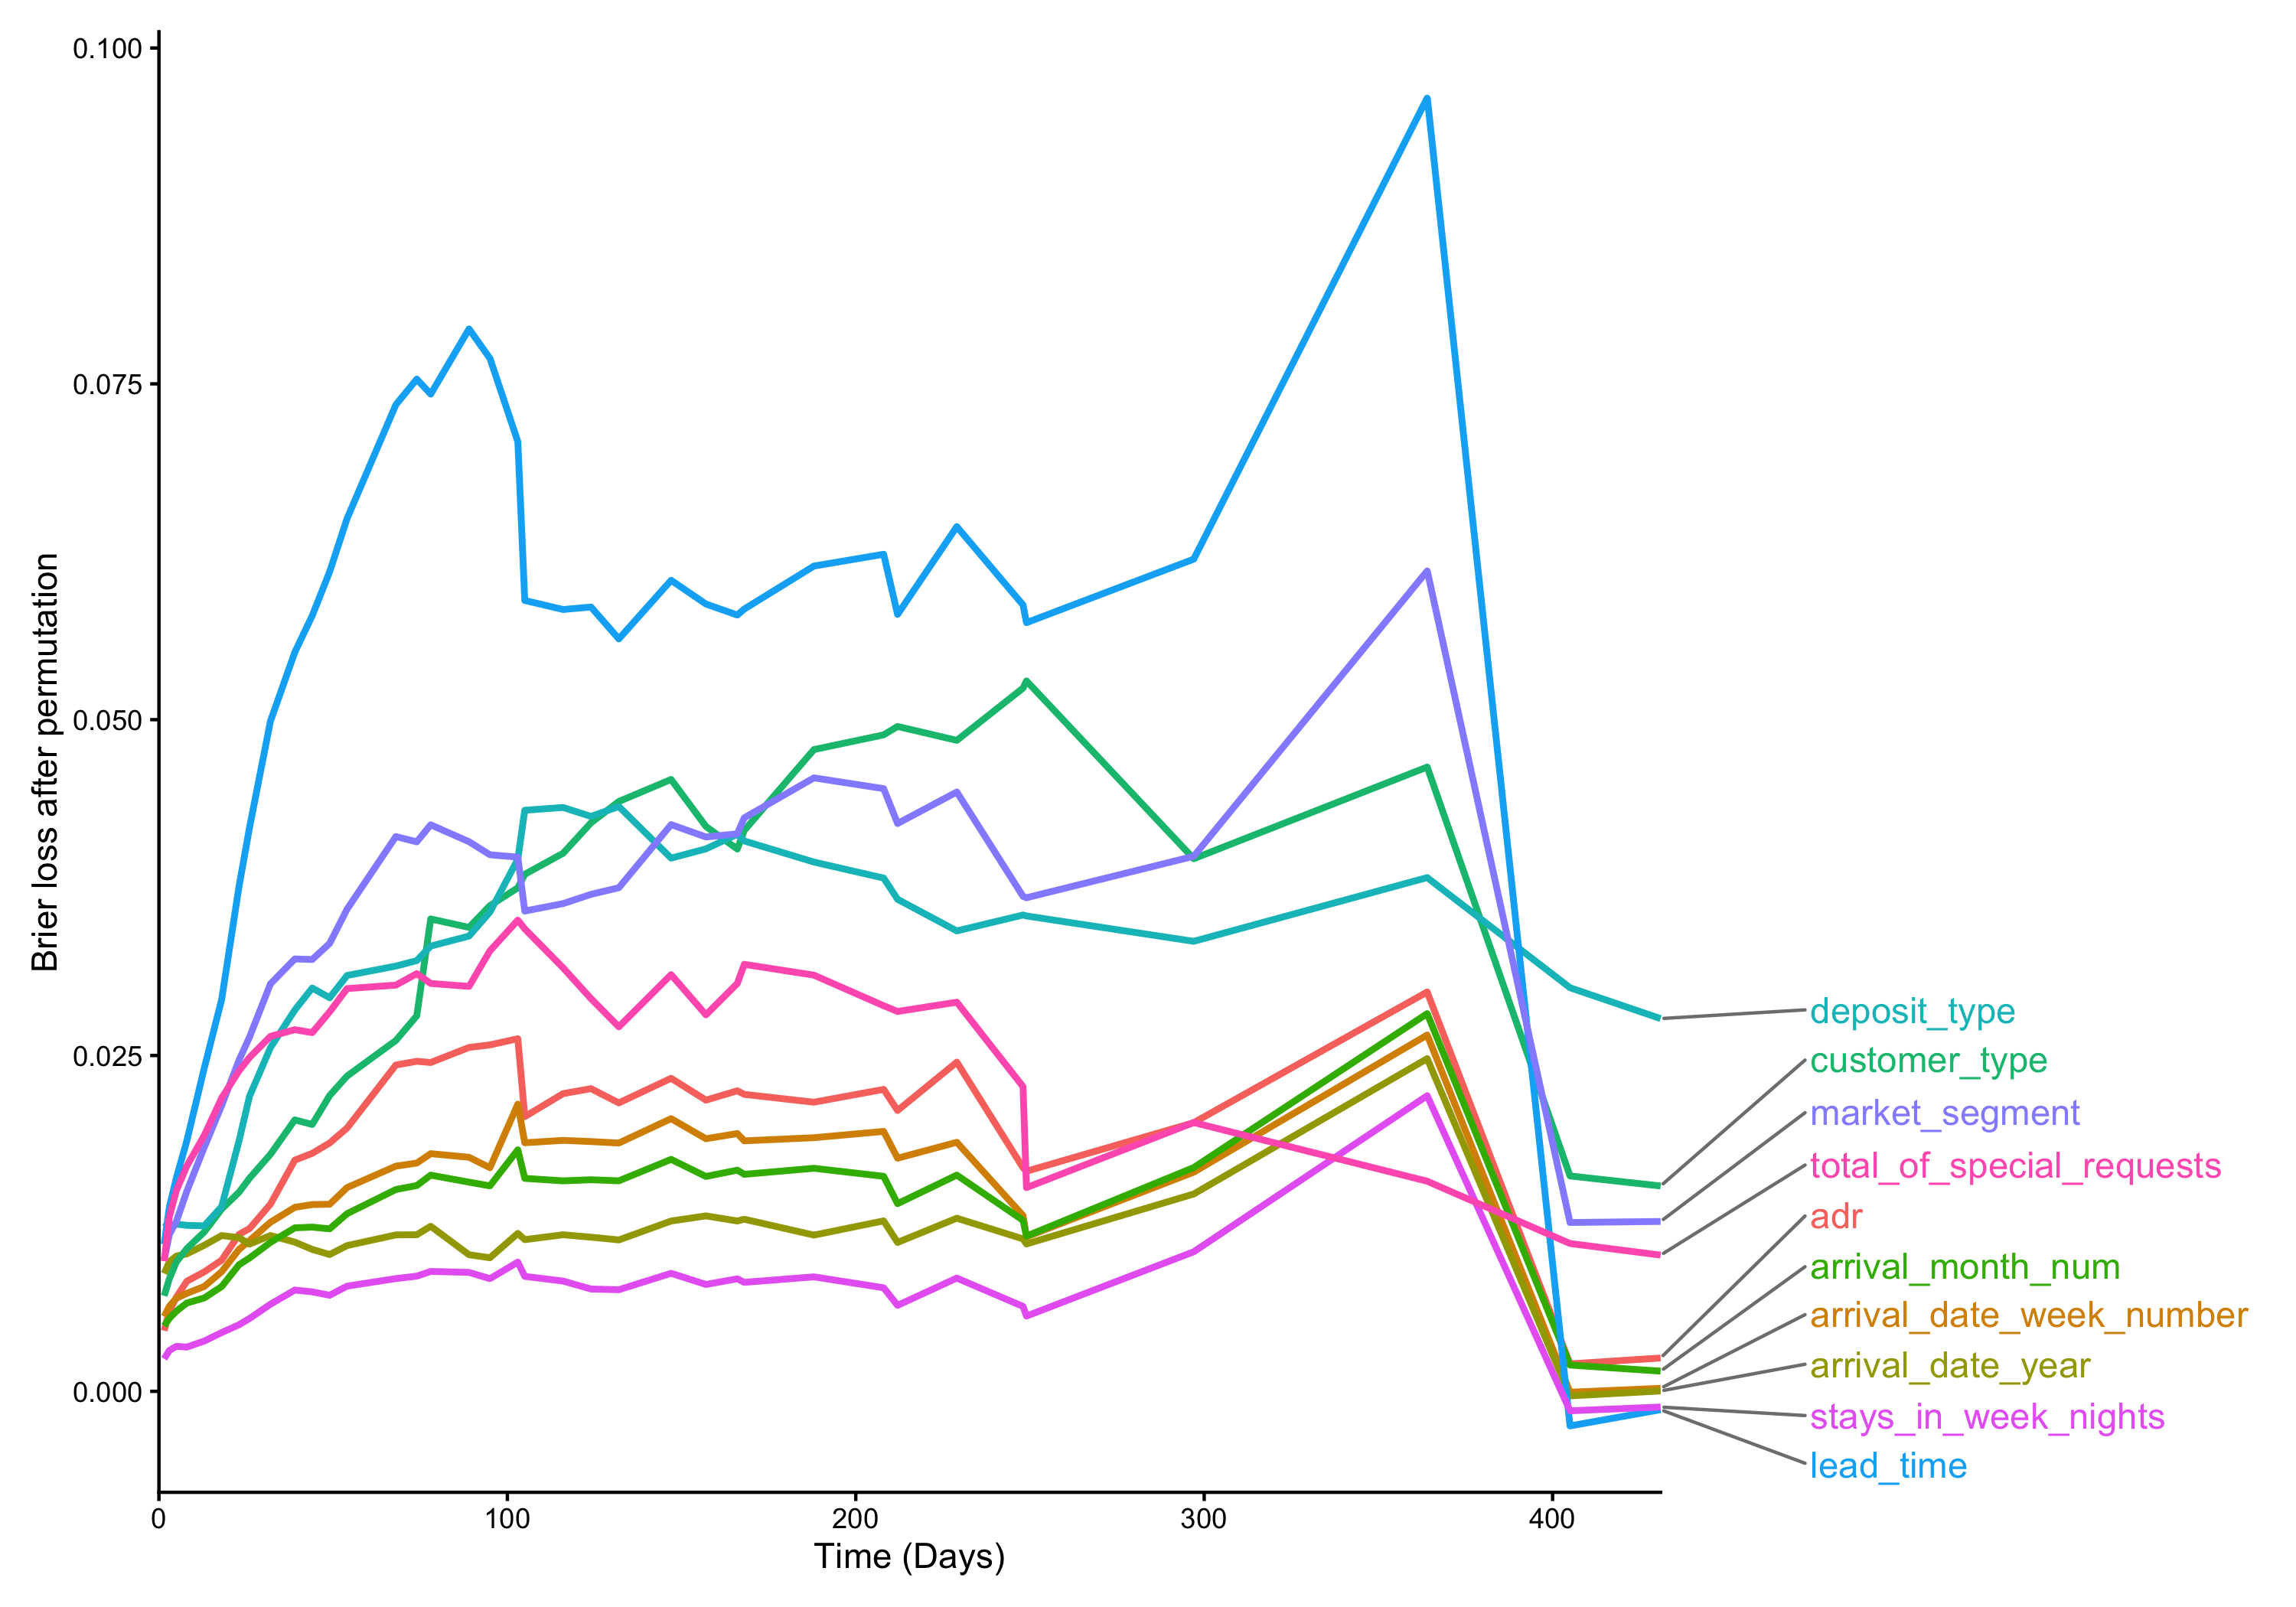
\includegraphics[width=0.9\textwidth]{fig_survpfi_ds1.png}
\caption{Time-dependent Survival Permutation Feature Importance (SurvPFI) for the Oblique RSF model on Dataset 1, measured as the delta in Brier loss over time.}\label{fig:survpfi_ds1}
\end{figure}

The analysis of Dataset 2, as depicted in Figure~\ref{fig:survpfi_ds2}, provides contrasting insights due to structural differences in the feature space—most notably, the absence of deposit-related variables. In this environment, \texttt{lead\_time} assumes absolute dominance in predicting cancellation hazard, with its importance compounding aggressively over time. Strikingly, in the absence of deposit constraints, the average daily rate (\texttt{adr}) emerges as the second most critical determinant of cancellation risk, indicating high price elasticity. The temporal rise in ADR importance confirms that prospective guests actively monitor pricing environments; as the check-in date approaches, guests holding reservations at higher ADRs exhibit a pronounced tendency to cancel, likely engaging in intertemporal arbitrage to secure lower rates elsewhere.

\begin{figure}[htbp]
\centering
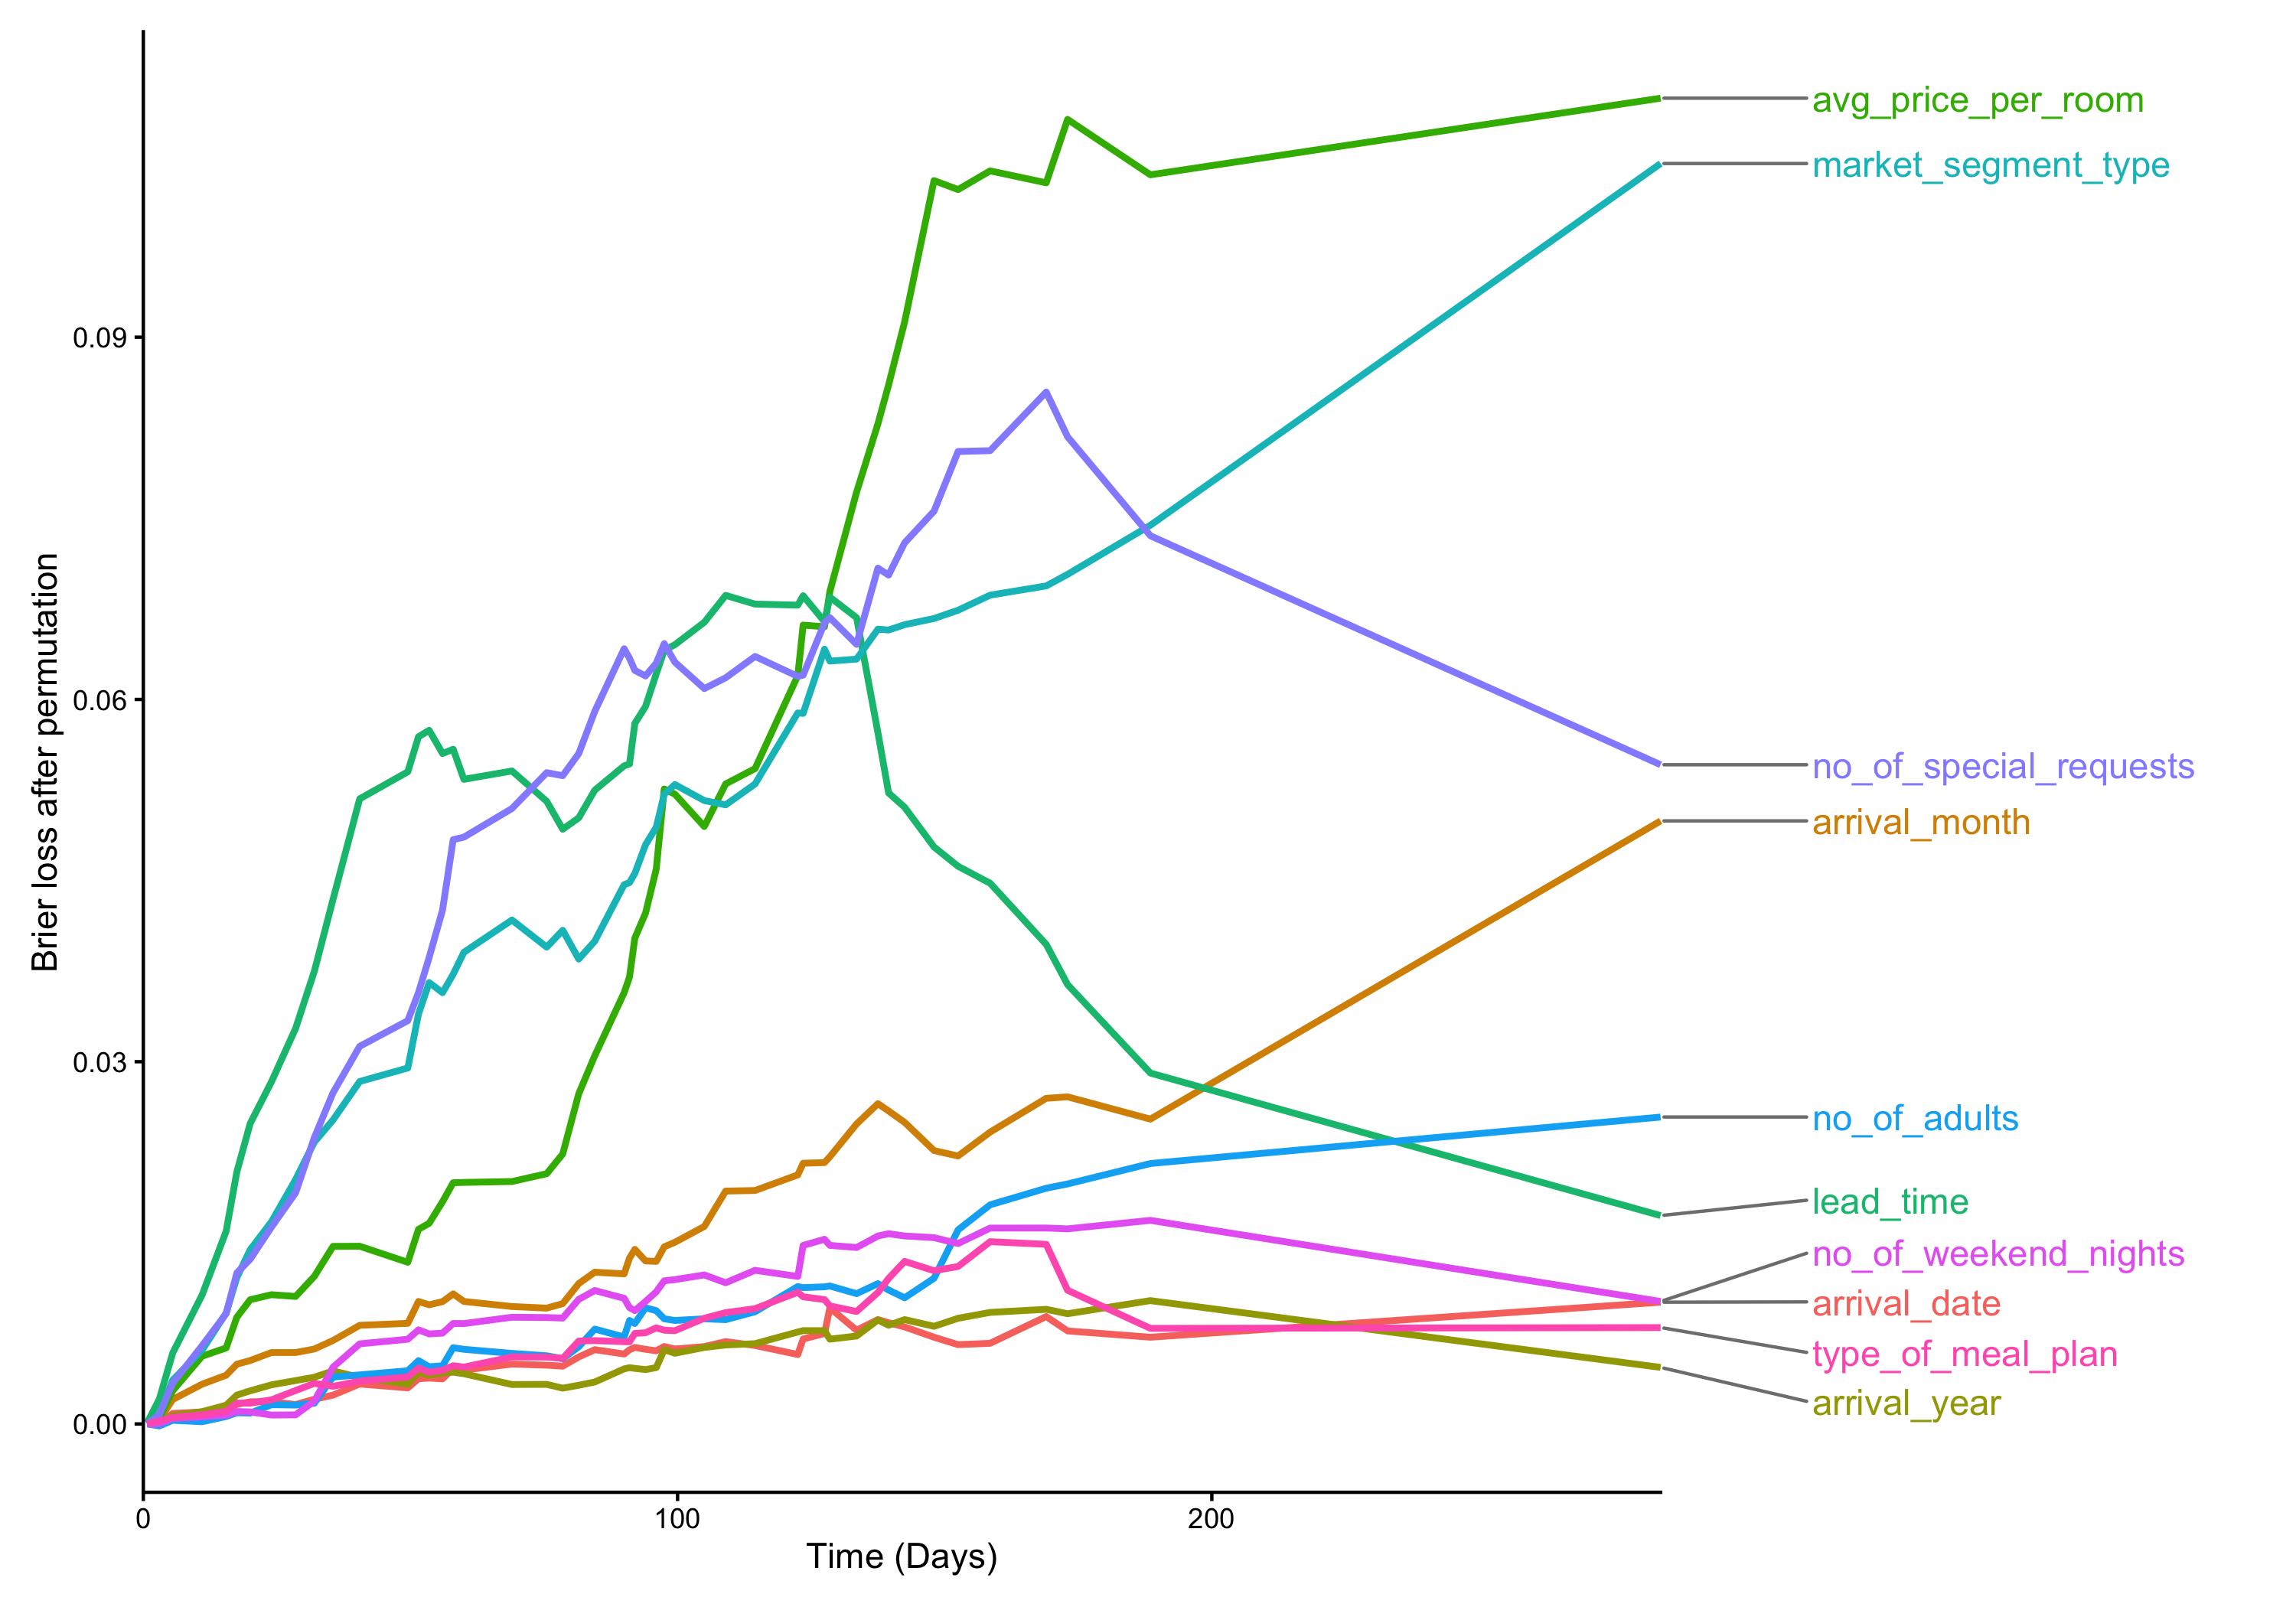
\includegraphics[width=0.9\textwidth]{fig_survpfi_ds2.png}
\caption{Time-dependent Survival Permutation Feature Importance (SurvPFI) for the Conditional Forest model on Dataset 2, highlighting the temporal dominance of lead time and price (ADR).}\label{fig:survpfi_ds2}
\end{figure}

While SurvPFI, adapted to survival analysis by \cite{langbein2025interpretable} based on the foundational permutation importance principles of \cite{breiman2001random}, delineates \textit{which} features drive predictive performance, it does not reveal the marginal effect of these features on the actual survival probability. To bridge this gap, we employ Partial Dependence Survival Profiles (SurvPDP) \citep{langbein2025interpretable}, which extends the partial dependence concept of \cite{friedman2001greedy} to the time-to-event domain. By marginalizing over the distribution of all other variables, SurvPDP isolates the average effect of varying a single feature's value across the entire temporal horizon.

Figure~\ref{fig:survpdp_ds1} presents the SurvPDP curves for the top six most influential features of the Oblique RSF model on Dataset 1. The \texttt{deposit\_type} profile is particularly striking: reservations with a \textit{Non Refund} policy exhibit a drastically lower baseline survival probability compared to \textit{No Deposit} bookings. This seemingly counterintuitive phenomenon is thoroughly documented in hospitality literature regarding this specific dataset, as non-refundable rates were heavily associated with speculative group bookings that were later cancelled en masse. Additionally, the \texttt{lead\_time} profile demonstrates a monotonic decline in survival probability as the booking window expands; reservations made over 200 days in advance suffer from significantly higher attrition rates. Finally, \texttt{market\_segment} reveals that bookings originating from \textit{Groups} or \textit{Online TA} (Travel Agents) maintain consistently lower survival probabilities than direct or corporate bookings, highlighting the lack of commitment inherent in platform-based or block reservations.

\begin{figure}[htbp]
\centering
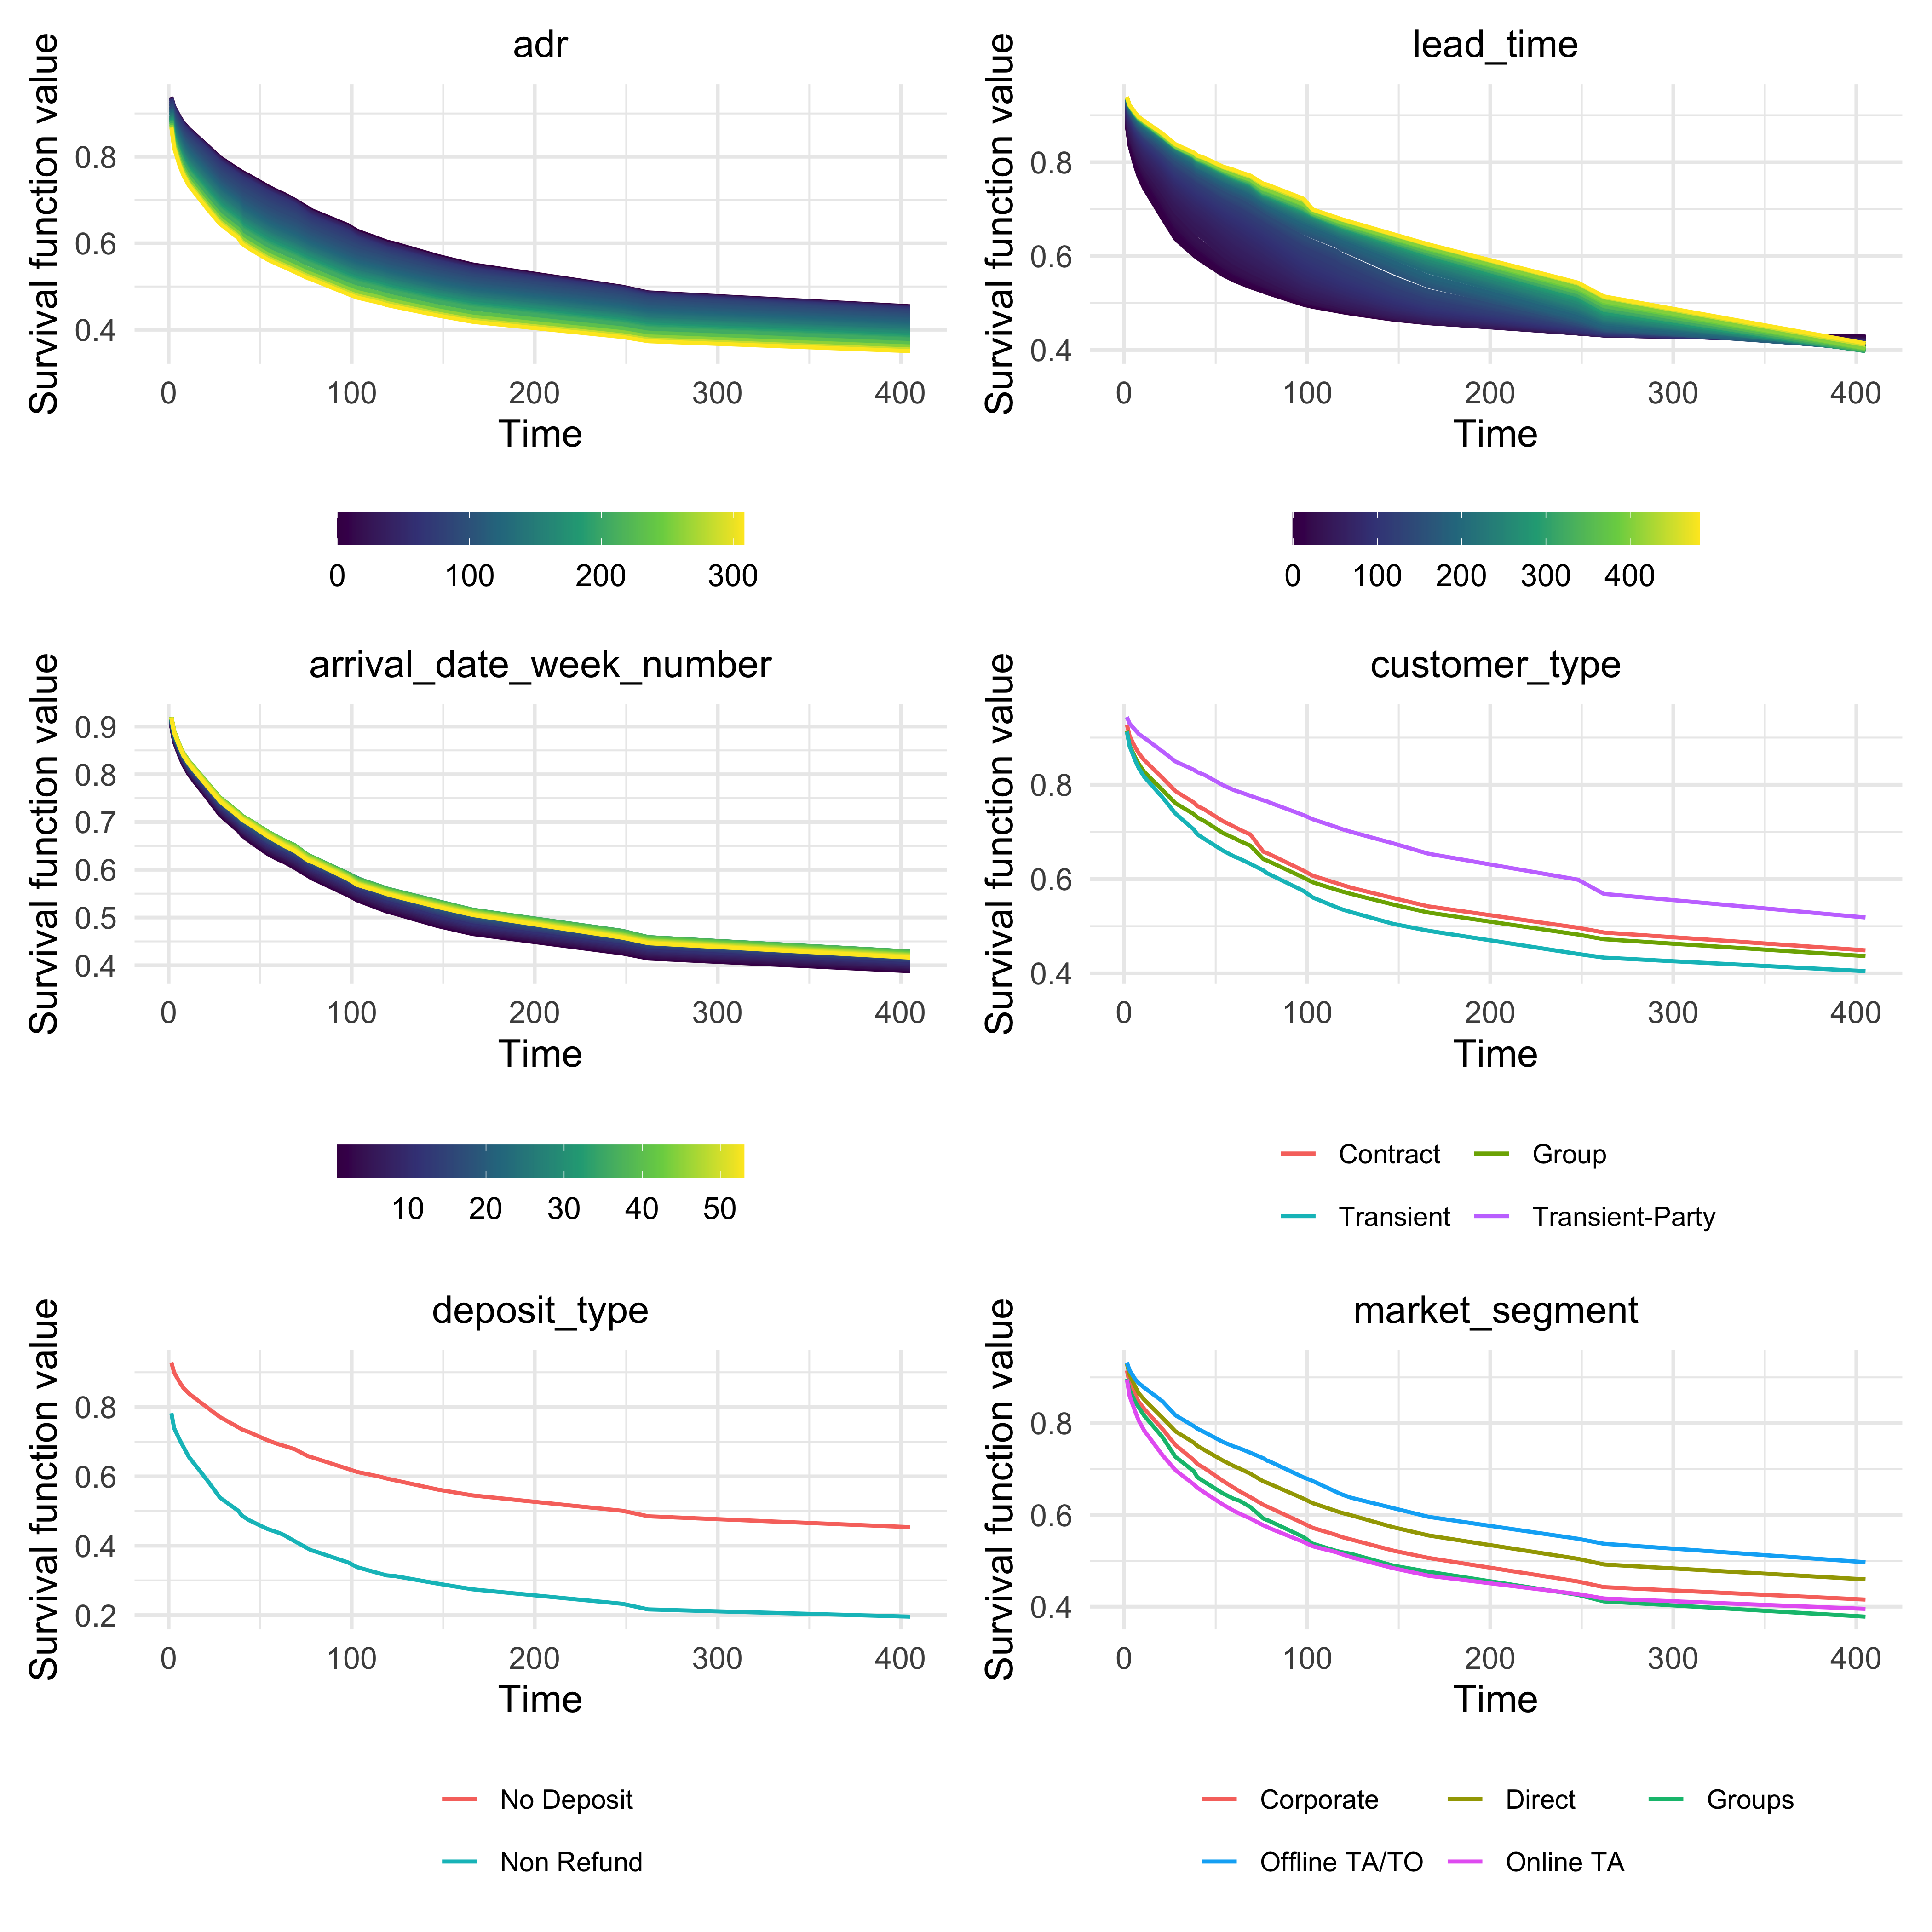
\includegraphics[width=0.9\textwidth]{fig_survpdp_ds1.png}
\caption{Partial Dependence Survival Profiles (SurvPDP) for the Oblique RSF model (Dataset 1). Each panel isolates the marginal effect of a specific feature's values on the survival (non-cancellation) probability over time.}\label{fig:survpdp_ds1}
\end{figure}

In Dataset 2 (Figure~\ref{fig:survpdp_ds2}), the Conditional Forest model's profiles underscore the structural absence of deposit policies. The \texttt{lead\_time} effect mirrors Dataset 1, reinforcing the universal rule that longer planning horizons breed higher cancellation risks. Crucially, the continuous profile for average daily rate (\texttt{adr}) provides granular insight into price sensitivity: higher daily rates systematically depress the survival probability curve. As time approaches the check-in date, the survival gap between low-priced and high-priced reservations widens, empirically validating that price elasticity drives late-stage cancellations. Furthermore, the \texttt{arrival\_month} and \texttt{market\_segment\_type} profiles capture seasonal variations and booking channel reliabilities, offering revenue managers actionable thresholds for dynamic overbooking and pricing strategies.

\begin{figure}[htbp]
\centering
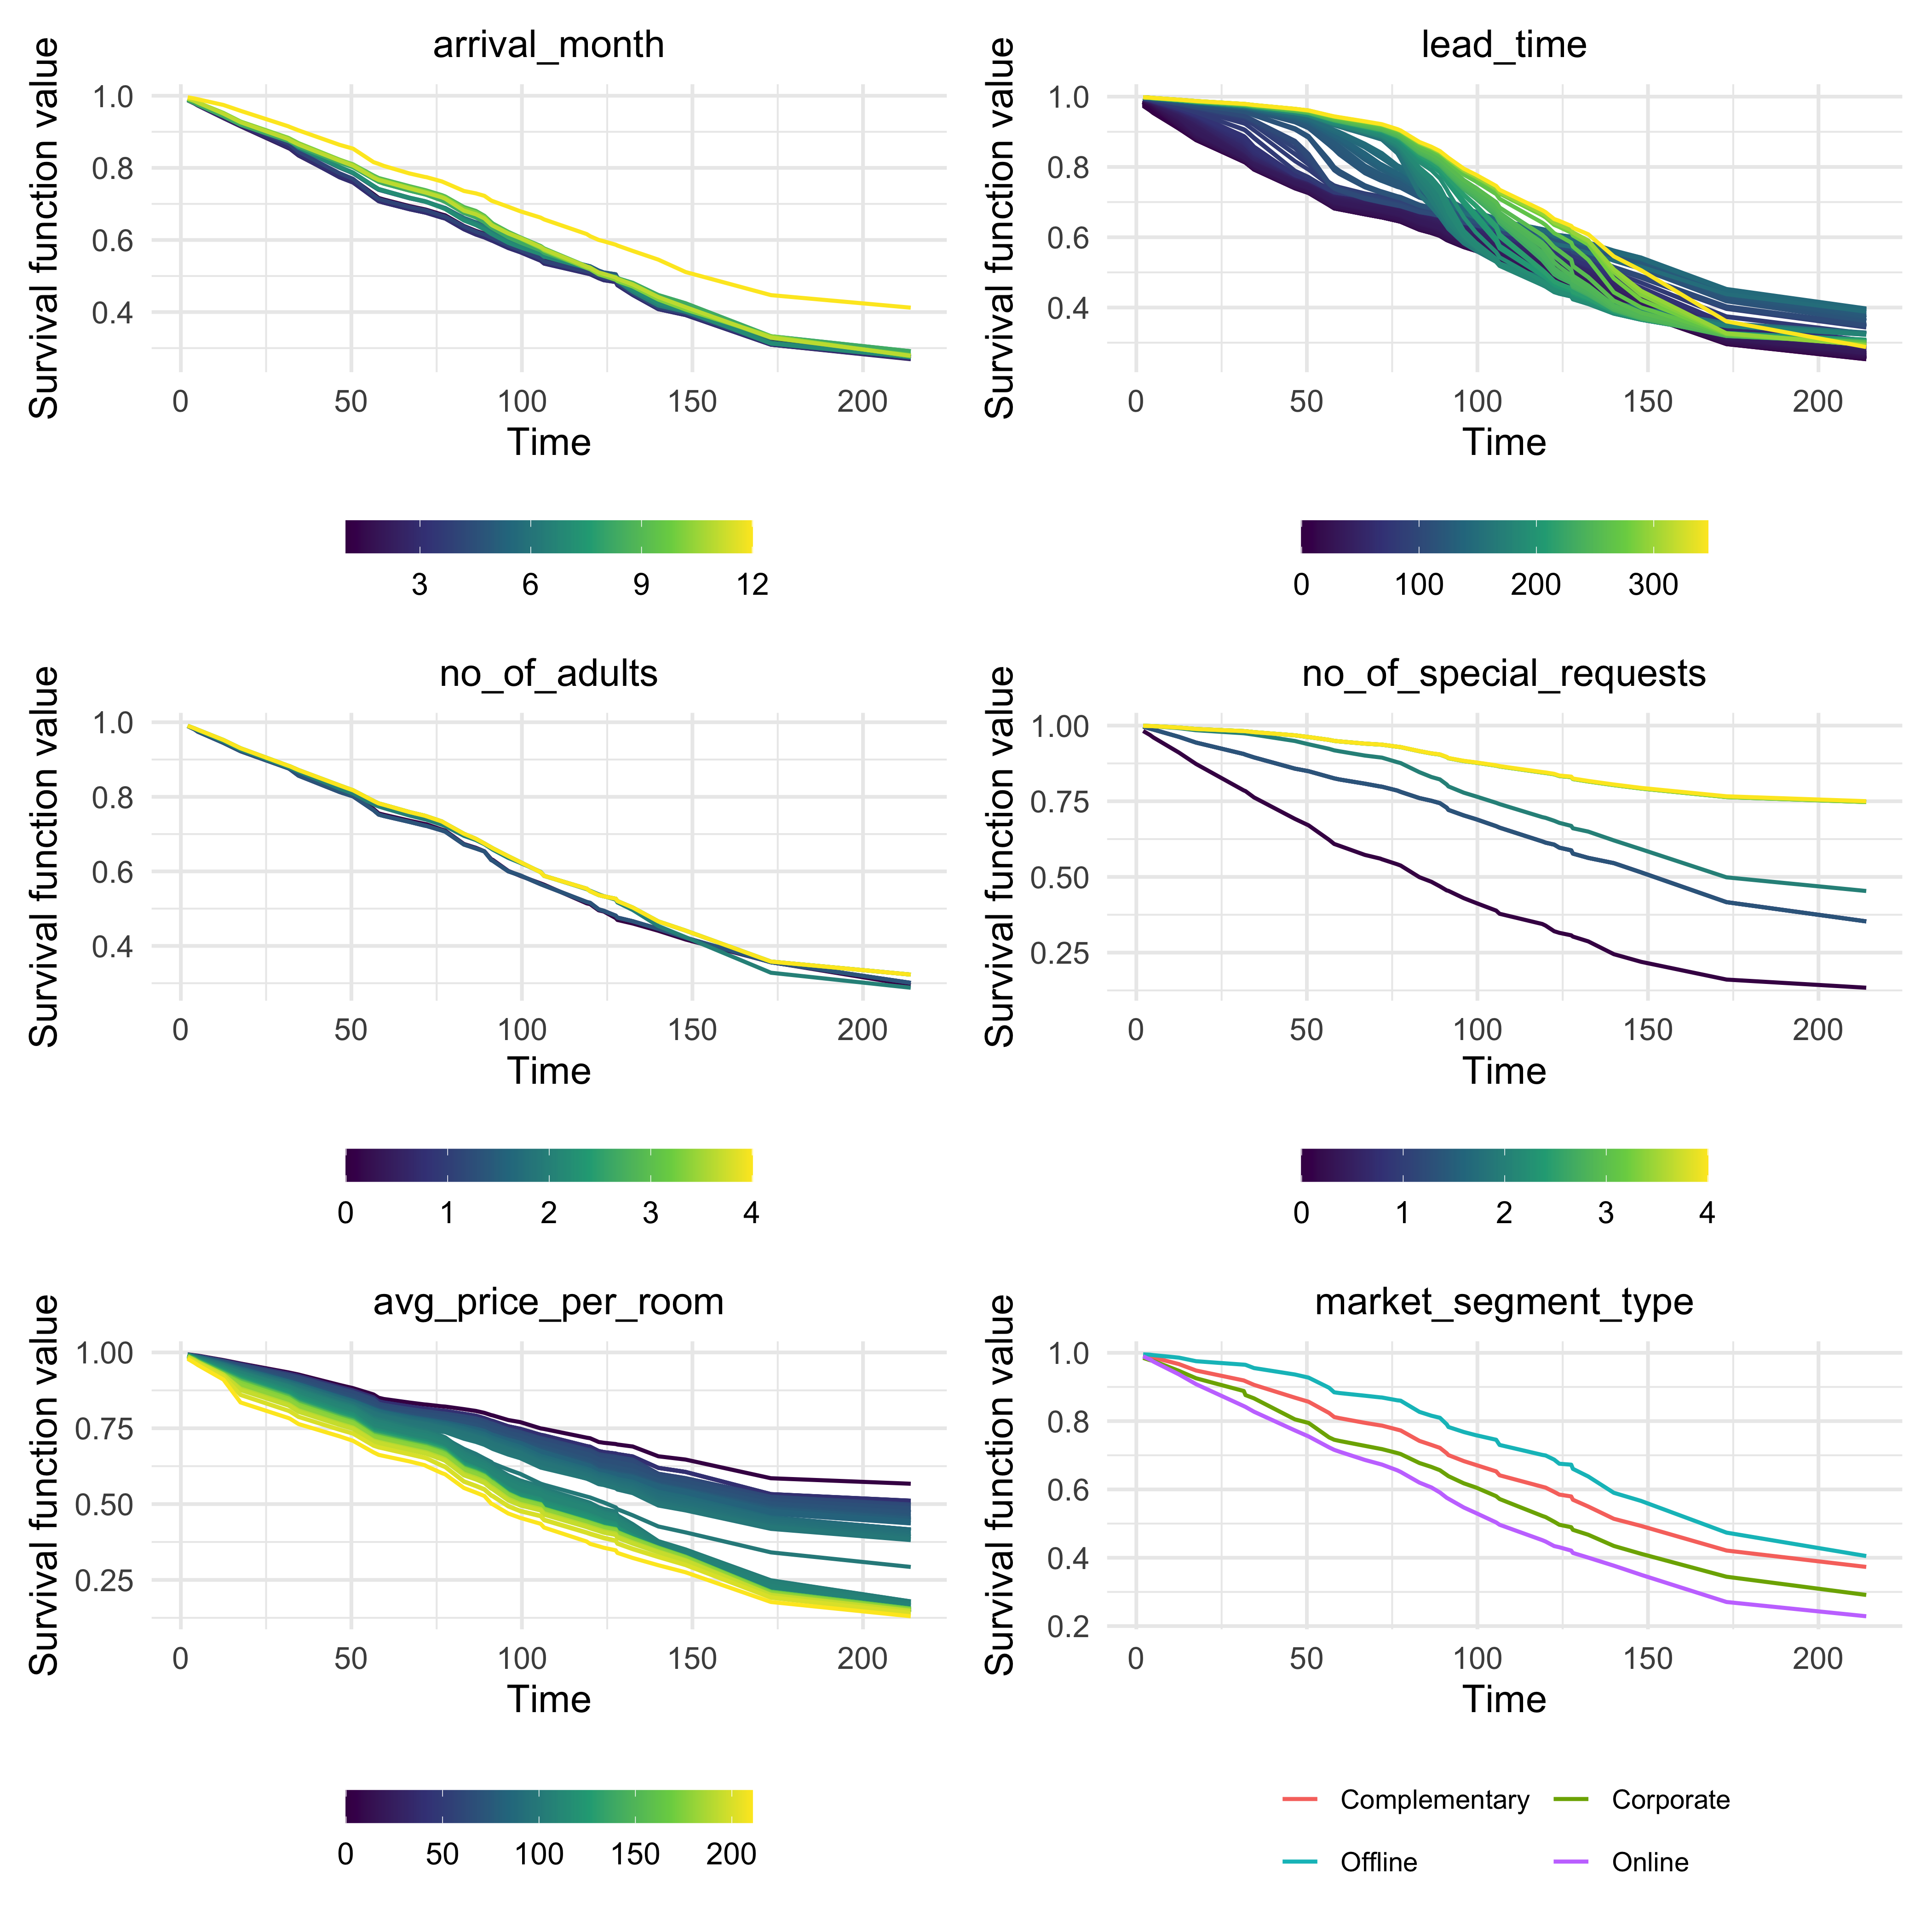
\includegraphics[width=0.9\textwidth]{fig_survpdp_ds2.png}
\caption{Partial Dependence Survival Profiles (SurvPDP) for the Conditional Forest model (Dataset 2), illustrating the marginal temporal impact of price (ADR), lead time, and other critical covariates.}\label{fig:survpdp_ds2}
\end{figure}

%%%%%%%%%%%%%%%%%%%%%%%%%%%%%%%%%%%%%%%%%%%%%%%%%%%
\section{Discussion} %%%%%%%%%%%%%%%%%%%%%%%%%%%%%%
%%%%%%%%%%%%%%%%%%%%%%%%%%%%%%%%%%%%%%%%%%%%%%%%%%%
\label{sec:discussion}

The empirical results of this study fundamentally advance the analytical frameworks utilized in hospitality revenue management. Previous literature \citep{antonio2017predicting, falk2018modelling, chen2023prediction} has predominantly framed booking cancellations as static binary classification tasks. While these conventional machine learning models can identify \textit{whether} a booking will be canceled, they inherently fail to capture the temporal dimension of the cancellation hazard. By restructuring the problem through the lens of survival analysis, this study provides a dynamic mechanism to estimate the evolving probability of cancellation as the check-in date approaches. While recent studies, such as \cite{mir2026decoding}, have begun exploring time-to-event modeling to investigate the behavioral timing of cancellations, our research uniquely bridges this survival framework with time-dependent XAI. This integration elevates complex predictive models from theoretical constructs to transparent, trustworthy, and actionable decision-support tools.

Consistent with earlier findings \citep{antonio2019big, yang2024predicting}, our analysis reaffirms that \texttt{lead\_time} and \texttt{deposit\_type} are dominant predictors of cancellation behavior. However, the integration of time-dependent XAI, namely SurvPFI and SurvPDP, extends these classical insights by mapping their marginal effects across the survival horizon. For instance, while \cite{liu2023hospitality} identified price sensitivity as a static risk factor, our SurvPDP analysis in Dataset 2 empirically visualizes how the influence of ADR compounds over time. We observe that reservations secured at higher rates experience a sharply accelerating cancellation hazard as check-in approaches, likely driven by guests monitoring the market for last-minute intertemporal arbitrage opportunities \citep{mir2026decoding}. While \cite{talal2025hotel} utilized standard XAI tools to decode the static behavioral drivers of cancellations, our SurvPFI approach pushes the boundaries of explainability by revealing how these behavioral drivers dynamically evolve over the booking window.

Moreover, this study highlights a critical trade-off in survival modeling: concordance versus calibration. While standard Random Survival Forests achieved high C-index scores by ranking risks effectively, they exhibited poor probability calibration as evidenced by high Brier scores. Conversely, Oblique RSF and Conditional Survival Forests provided highly calibrated probabilities. For revenue managers configuring dynamic overbooking limits, accurately calibrated probabilities—rather than mere ordinal rankings—are indispensable \citep{ampountolas2025predicting}. Furthermore, \cite{liu2025explainable} recently highlighted that advanced ensemble models in hotel cancellation forecasting often suffer from limited explainability, hindering their practical alignment with business objectives. The deployment of SurvPDP in our study explicitly resolves this transparency deficit by providing interpretable, continuous risk curves that can be directly mapped to revenue management strategies.

The anomalies detected in the deposit type feature in Dataset 1—where \textit{Non Refund} bookings exhibited paradoxical cancellation rates—align with dataset-specific observations noted by \cite{antonio2019big}, stemming from speculative block bookings. The SurvPDP framework successfully isolated and exposed this structural anomaly, demonstrating the vital necessity of applying XAI to validate model behavior before deployment in automated pricing systems.

%%%%%%%%%%%%%%%%%%%%%%%%%%%%%%%%%%%%%%%%%%%%%%%%%%%
\section{Conclusion} %%%%%%%%%%%%%%%%%%%%%%%%%%%%%%
%%%%%%%%%%%%%%%%%%%%%%%%%%%%%%%%%%%%%%%%%%%%%%%%%%%
\label{sec:conclusion}

This research demonstrates the efficacy of integrating advanced machine learning survival models with time-dependent XAI to predict and interpret hotel booking cancellations. By transitioning from static classification to dynamic time-to-event modeling, we evaluated 10 distinct survival algorithms across two distinct datasets. Our benchmarking revealed that Oblique Random Survival Forests and Conditional Survival Forests achieve an optimal balance between discriminative power, measured by the C-index, and probability calibration through IBS and RCLL metrics, making them highly suitable for deployment in dynamic revenue management systems.

Beyond predictive performance, the application of SurvPFI and SurvPDP frameworks successfully demystified the temporal dynamics of these black-box models, directly addressing the critical need for algorithmic transparency, verification, and responsible AI governance \citep{meske2022explainable}. The explanations quantified the non-linear, time-varying impacts of lead time, ADR, and deposit policies on the evolving cancellation hazard. These insights equip hotel operators with the granular, actionable intelligence required to dynamically adjust overbooking capacities, tailor cancellation penalties, and optimize pricing strategies as the booking window matures.

A limitation of this study is the absence of formal statistical significance testing (e.g., Diebold-Mariano tests or bootstrap confidence intervals) for comparing model performance metrics, restricting the comparisons to point estimates. Furthermore, the reliance on historical, tabular booking data without incorporating exogenous macroeconomic indicators or real-time competitor pricing represents another limitation. Future research should explore the integration of time-varying covariates, such as dynamic market prices and real-time flight demand, into deep survival analysis architectures to further refine the accuracy of temporal cancellation forecasting.

\backmatter

\section*{Declarations}

\noindent \textbf{Funding} This research received no external funding.\\

\noindent \textbf{Conflict of interest} The authors declare no competing interests.\\

\noindent \textbf{Data availability} The datasets used in this paper are publicly available online.\\

\noindent \textbf{Code availability} The codes for reproducing the experiments performed are accessible in the following repository: \url{https://github.com/mustafacavus/hotel-cancellation-survival}.\\

\bibliography{sn-bibliography}

\end{document}
